% !Mode:: "TeX:UTF-8"
\renewcommand{\b}{\boldsymbol}

\chapter{基于可微ODE-Net的高时延工业多输入输出系统预测}
在复杂过程工业系统控制研究领域中,基于传统控制理论的系统辨识及控制器设计方法受限于系统复杂性难以适用。
而基于强化学习的无模型控制策略学习方法虽然不受系统复杂性的影响,但需要与环境之间不断进行交互反馈,因此同样不适用于试错代价极其高昂的工业场景。
随着大数据采集与处理技术的不断进步,很多企业会在复杂工业设备上安装大量传感器以监测工业系统的实时运行过程。
构建时序预测模型并利用采集到的数据集进行训练,然后采用基于预测模型的系统优化及控制策略解决复杂系统的决策难题~\cite{Yuan2020,Member2019,wu2020optimization}。
为了实现面向复杂工业系统的建模与预测,需要对复杂工业系统的内在特性进行深入分析,我们发现此类系统通常具有以下典型特征:

a)\ \textbf{非线性系统动力学:}大多数工业系统都有极其复杂的高阶动力学方程,它们不是仿射系统或线性系统。

b)\ \textbf{系统的部分观测性}:从传感器或其他可用方法提取的信息是不完整的。特别是,在这样的系统中存在许多未知的隐变量。

c)\ \textbf{长延迟的影响}:系统状态受外部输入或在很长一段时间之前发生的内部状态的影响。

d)\ \textbf{连续时间演化}:由于真实的工业系统遵循各种物理规律,它们的时间演化可以用CT微分方程表示。

对于上述复杂工业系统特点,许多工业界和学术界的研究人员通过构建不同预测模型来解决这些问题。其中,数据驱动方法为建模复杂工业过程最常用的技术\cite{larsson2002identification}。
特别地,在基于数据的连续时间系统预测及辨识领域中,研究人员主要利用采样于真实系统的有噪数据来拟合高阶微分方程。
然而,这种方法不适用于建模部分可观测系统(Partially Observed System)和极端复杂的工业系统.
伴随着深度神经网络技术的不断发展,得益于其强大的特征表示能力和可扩展的参数结构,深度学习在解决复杂工业系统的预测及分析问题时被广泛使用。如时间序列预测~\cite{Member2019,Essien2020,9161367,9522017,neu2021systematic}、设备异常检测等~\cite{9326384}。
然而,现有的大多数基于深度学习的系统建模及预测方法都是基于离散时间的,忽略了系统的连续时间特性。从模型结构与系统本体的一致性角度来看,忽视系统本身具备的物理先验特性会增加模型的自由度及拟合难度,进而限制了模型精度。
% The above features of a thickening system create challenges for predictive control. There are a number of studies addressing these challenges. 
% Data-driven methods are emerging as one of the most successful techniques for modeling complex processes~\cite{larsson2002identification}. 
% Traditional data-based CT system prediction methods focus on fitting high-order differential equations based on sampled noisy data from real systems. 
% However, they lack the ability to cope with partially observed and extremely complex system dynamics.
% Recent advances of deep neural networks (DNNs) have shown their strengths in addressing these issues owing to their strong feature representation abilities and scalable parameter structures, leading to the wide usage of DNNs in computer vision\cite{voulodimos2018deep,ma2020data, ma2021sesf}, natural language processing~\cite{young2018recent,9260162}, time series prediction~\cite{Member2019,Essien2020,9161367,9522017,neu2021systematic}, and fault diagnosis~\cite{9326384}. However, most DNN-based system-modeling methods are based on discrete time, disregarding the CT properties of a system. The lost prior information from physical insights undoubtedly leads to the deterioration of the model accuracy. 

另一方面,利用本章节所介绍的复杂系统预测模型,可以从两方面辅助系统控制的研究:

首先,模型的预测结果能够为基于模型的控制算法提供短期预测功能,例如模型预测控制(Model Prediction Control, MPC)~\cite{Member2019}。在MPC方法中,预测模型提供了动力系统会如何受控制输入影响的先验知识,从而将系统最优控制近似为了序列优化问题。
其次,预测模型可以模拟系统在长控制输入信号下的系统输出~\cite{Demeester2020SystemIW},因此可以作为验证系统控制策略可行性的试错仿真场景。在复杂的过程工业系统控制领域中,验证控制器的性能和安全性是有极其必要的。
与短期预测相比,系统输出模拟需要预测模型有更高的稳健性和稳定性来提供长期的无反馈开环预测。
然而,在现有围绕工业系统预测的方法研究中,很少有关注于如何设计预测模型以适用于短期和长期预测,进而服务于MPC控制及系统仿真。

针对上述工业系统存在的复杂特性以及长短期预测需求,本章节以ODE-net作为模型骨架结构,从连续时间域角度拟合复杂工业系统的动态过程,由此提出了一种由序列编码器、状态解码器和导数模块组成的深度连续时间(Continuous Time, CT)网络,以端到端的方式学习工业系统输出的自回归变化过程和输入对输出的非线性影响。
以实现给定历史系统运行轨迹及未来系统控制输入序列情况下,预测系统输出的未来变化。

% 因此,本章将以ODE-net作为模型骨架结构,从连续时间域角度拟合复杂工业系统的动态过程,以实现给定历史系统输出序列及未来系统控制输入序列情况下,预测系统输出的未来变化。
具体地,由于工业系统往往存在长时间的系统延迟,因此本章节引入序列编码器以从历史系统运行轨迹中提取特征。
在预测时,该方法构建了基于深度连续时间状态空间的导数模块。该模块相比于传统的离散序列模型,如RNN等。更适用于建模系统在连续时间域下的非线性演化,并且在模块中通过引入隐状态可以辅助推断系统的不可观测信息。
最后,本方法将非平稳系统和平稳系统概念融入在模型的导数模块设计中,可以有效解决系统的短期和长期预测问题。
% 通过将历史系统轨迹和任意长度的系统输入输入到模型中,解决了短期和长期预测问题。然后预测未来的系统输出。
本章研究在工业系统预测领域有三个方面贡献:
%%%%%%%%%%%%%%%%%%%%%

a)\ 提出了一种新的基于深度学习的工业系统连续时间预测模型。深度学习网络由三个部分组成:序列编码器、状态解码器和导数模块。

b)\ 基于平稳系统和非平稳系统概念,本章设计了两种导数模块,分别处理短期和长期预测任务。
%The analysis and experimental comparison are presented.

c)\ 利用来源于某真实铜矿场中膏体浓密机的历史运行数据验证了本章提出方法的有效性。结果表明,该模型在预测具有非线性和高时滞特性的浓密机系统时具有较好性能。此外,本章节还进行了部分消融研究,以评估模型中每个模块的有效性。

本章节内容组织如下:
~\ref{sec:formulate}节主要介绍了预测问题的形式化表述。
~\ref{sec:model}节介绍了本章所述的连续时间深度预测模型。
% ~\ref{sec:derivative}节具体介绍了面向短期预测和长期预测的两种导数模块定义方法。
% ~\ref{sec:interpolation}节具体介绍了用于连续化系统输入序列的并行插值方法。
% ~\ref{{sec:train}介绍了用于连续化系统输入序列的并行插值方法
% We next present the CT deep sequential model in Section~\ref{sec:CTDSM}. 
\ref{sec:case}节介绍了将本章所述方法用于膏体浓密机系统预测问题的实验结果。
\ref{sec:conc}节对本章工作进行了总结,并讨论了未来的研究方向。

\section{问题形式化表述}
\label{sec:formulate}
在复杂工业系统中,系统输出量定义为$\b y(k) \in \mathbb{R}^n$,
其中$k$为采样时间指标。将影响系统输出量的系统控制输入量定义为$\b x(k)\in \mathbb{R}^m$。
在诸多复杂工业场景中,系统输入对系统输出的影响本质上是非线性、高时滞的。且由于监测技术的限制,系统的一些关键参数无法获得,系统的观测空间往往是不完备的,
同时,观测数据会受到环境噪音以及系统本体中未知扰动的干扰。
此类复杂特性使得传统系统辨识方法\cite{larsson2002identification}或预测模型\cite{box2015time}难以对复杂工业系统进行有效的学习。
因此本章采用基于深度学习的黑箱数据驱动方法建模复杂系统的状态空间模型,使模型能够利用序列数据推断系统的隐状态。
进一步地,将系统预测问题建模为在已知未来系统输入和历史系统运行轨迹下估计未来系统输出。
% we formulate the problem as a sequential prediction structure with symbolic modules:
我们首先定义系统的历史输入序列为 $\boldsymbol X_p^{N_x}=[\boldsymbol x(-N_x),\boldsymbol x(-N_x+1), \dots, \boldsymbol x(-1)]$, 历史系统输出为 
$\boldsymbol Y_p^{N_y}=[\boldsymbol y(-N_y),\boldsymbol y(-N_y+1),\dots, \boldsymbol y(-1)]$,系统的未来输入为 $\boldsymbol y_f^{M}=[\boldsymbol y(0),\boldsymbol y(1),\dots,\boldsymbol y(M-1)]$,模型需要预测系统的未来输出$\boldsymbol Y_f^{M}=[\boldsymbol y(0),\boldsymbol y(1),\dots,\boldsymbol y(M-1)]$。
其中,$\boldsymbol X_f^{M}$之所以已知,是因为在MPC控制及系统仿真问题中,系统输入是已知的。
序列预测问题可用如下符号及公式表示:
% we reformulate the thickening system prediction problem as a sequential prediction structure to improve the accuracy of multi-step predictions:
\begin{equation}
\label{equ:discrete_seq2seq}
\left\{
\begin{aligned}
&\boldsymbol{h}(0) = \mathcal{F}(\boldsymbol X_p^{N_x}, \boldsymbol{Y}_p^{N_y}), \\
&\boldsymbol{H^M} = D(\boldsymbol{h}(0), \boldsymbol {X}_f^{M}),\\
&\boldsymbol{y}(k) = g(\boldsymbol{h}(k)),
\end{aligned}
\right.
\end{equation}

模块$\mathcal{F}(\cdot)$ 用于估计初始隐状态 $\b h(0)$,该隐状态携带了历史序列 $\boldsymbol X_p^{N_x} \text{ 和 } \boldsymbol Y_p^{N_x}$的信息。
构建合理的模型$D(\cdot, \cdot)$,即可利用初始的隐状态以及未来的系统输入,估计完整的系统状态序列$\b H^M$。序列中的每个隐状态$\boldsymbol h(k)$携带了、或编码了系统在$k$时刻的系统信息。另外,通过非线性函数$g(\cdot)$解码$\boldsymbol h(k)$即可得到估计的系统输出。
%%%%%%%%%%%%%%%%%%%%%%%
% seeking help: 我们扩展了\eqref{equ:discrete_state_space}中的单步预测到预测系统的序列输出. 被优化的loss 来源于整个预测序列各个位置loss的累计。
%We generalize the single-step prediction in \eqref{equ:discrete_state_space} to predicting sequential system outputs.
%The losses at all of the positions from predicted sequence are accumulated to construct complete supervised loss.
%Optimized loss is derived from the accumulation of losses at various positions in the predicted sequence.
% The loss function is optimized with grand total of the whole prediction sequence.
%%%%%%%%%%%%%%%%%%%%%%%
% For neural network based implementations, we sets  $M$ as a changeable parameter among training and inference phases. 

公式 \eqref{equ:discrete_seq2seq}类似于自然语言处理领域的Seq2Seq模型~\cite{Weiss2017Sequence},将三个序列$\boldsymbol X_p^{N_x}$, $\boldsymbol{Y}_p^{N_y}$,和 $\boldsymbol {X}_f^{M}$映射为被预测的系统输出序列$\hat {\boldsymbol {Y}}_f^{M}=[\hat{\boldsymbol {y}}(1),\hat{\boldsymbol y}(2),...\hat{\boldsymbol y}(M)]$。
然后,相比于机器翻译等序列转换任务,输入输出系统预测任务要求对于$\boldsymbol{h}(k)$的计算只能依赖于$\{\boldsymbol h(i), i\leq k-1\}$和$\boldsymbol{X}_{f}^{k}=\{\boldsymbol x(i), i\leq k-1\}$,
这样的限制促使本章在模型框架设计时采用自回归系统。

为了在预测模型中构造一个合理有效的模块$D$,一种简单有效的解决方案是采用单步自回归的离散时间状态空间模型 \cite{4019326}:
% From the perspective of discrete-time setting, a thickening system with long time delay and incomplete observations can be formulated by a state space model~\cite{4019326} which introduces hidden state $\boldsymbol h(t)$:
\begin{equation}
\label{equ:discrete_state_space}
\boldsymbol{h}(k)=d\big(\boldsymbol{h}(k-1), \boldsymbol{x}(k-1)\big),
\end{equation}
\begin{equation}
\boldsymbol{y}(k)=g(\boldsymbol{h}(k)),
\end{equation}
其中隐状态$\boldsymbol{h}(k)$将系统的历史轨迹编码为紧密、定长的向量。
系统控制输入的影响可以看作是对系统当前隐状态的单步非线性变换。
当给定某一时刻输入$\boldsymbol{x}(k-1)$和上一时刻隐状态$\boldsymbol{h}(k-1)$时,模型可以立即预测新的隐状态$\boldsymbol{h}(k)$。
一些先前的研究~\cite{CHAI201661}~\cite{KIM2004403}表明,大部分过程工业系统的运行本质为物理变化或化学变化,系统的动态过程更适合建模为连续域下的微分方程。
因此,本章遵照工业系统的先验知识,构建参数化连续时间微分方程模型,以拟合隐状态的一阶导数:
\begin{equation}
    \label{equ:derivative_model}
%\small
    \dot{\boldsymbol h}(t) = d(\boldsymbol{h}(t), \boldsymbol x(t)).
\end{equation}
在此处,离散下标$k$被替换为连续时间下标$t$以表示$\boldsymbol{h}(t)$的变化为连续时间过程。
对于复杂系统的预测模型可以进一步表示为式\eqref{equ:discrete_seq2seq} 和式 \eqref{equ:derivative_model}。
本章节的目标是利用收集得到的系统运行轨迹数据,对 上述模型中的各个参数化模块进行学习,包括序列编码器$\mathcal{F}(\cdot)$、连续时间导数模块$d(\cdot,\cdot)$和状态解码器$g(\cdot)$。
\section{基于ODE-net模型的多输入输出系统预测模型}
\label{sec:model}
本章采用集成的深度神经网络以参数化拟合公式~\eqref{equ:discrete_seq2seq}和~\eqref{equ:derivative_model}.
图~\ref{fig:model_structure}展示了网络中包含的各个组件及其连接。
对于给定条件范围内的历史序列轨迹 $\boldsymbol{X}_{p}^{N_{x}}$ 和 $\boldsymbol{Y}_{p}^{N_{y}}$,以及预测范围 内的系统输入序列$\boldsymbol{X}_{f}^{M}$,模型输出$\hat{\boldsymbol{Y}}_{f}^{M}$以近似估计系统输出 $\boldsymbol{Y}_{f}^{M}$。
% We separately introduce a recurrent neural network (RNN) network to encode historical system trajectories to the initial hidden state and an ODE system to describe the state space model in the given time range.

该模型的预测过程分成以下几个步骤。
首先, 采用基于循环神经网络的\textbf{序列编码 编码器},将历史轨迹序列$\boldsymbol{X}_{p}^{N_{X}}$和$\boldsymbol{Y}_{p}^{N_{Y}}$编码为隐状态$\b h(t_0)$。
然后,将$\b h(t_0)$作为预测阶段待求解常微分方程的初始状态。
常微分方程的一阶导数由模型中的\textbf{导数模块}定义,模型将隐状态$\b h(t)$和连续时间域中任意时刻的外部控制信号$\b x(t)$作为输入,以估计隐状态$\dot{\b h}(t)$的瞬时导数。
模型中引入的\textbf{并行样条插值}模块将离散的外部输入序列$\boldsymbol{x}_{f}^{M}$插值为连续时间形式$\b x(t)$以作为导数模块的输入。
接下来,利用ODE求解器求解基于初始状态$\b h(t_0)$和导数模块定义的常微分方程,可以得到时间范围$[0\leq t \leq t]$内的系统隐状态$\b h(t)$。
% The derivative of the hidden state with respect to the time variable $ \dot{\b h}(t)$ in the state space model is determined based on a neural network differential function $\b d(\b h(t), t)$. 
最后,模型利用基于多层感知器(MLP)网络的\textbf{状态解码器},将求解出的隐状态$\b h(t)$映射为待预测的系统未来输出$\hat{\boldsymbol{Y}}_{f}^{M}$。
% We then provide a detailed introduction of each network module. 
接下来,本章将详细介绍所述模型的每个模块的技术细节。

\begin{figure}[t]
    \centering
    %\setlength{\abovecaptionskip}{-0.1cm} 
    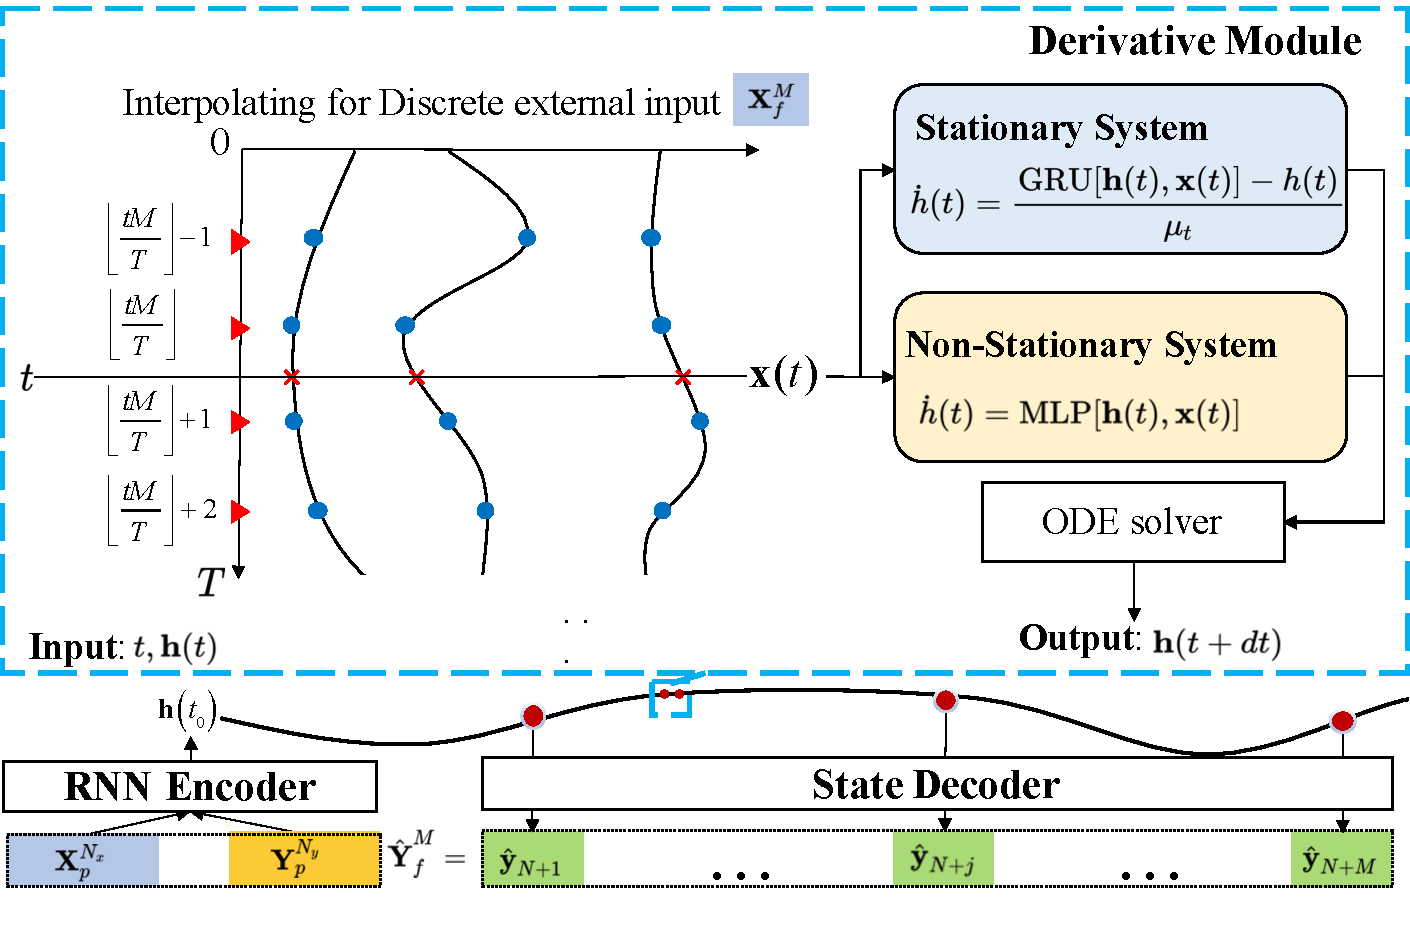
\includegraphics[width=1.0\linewidth]{figures/chapter3/model.pdf}
    \caption{
    基于ODE-net模型的输入输出系统预测模型整体结构
    % The optimized loss is defined according to accumulative errors in the complete predicted sequence. 
    }
    \label{fig:model_structure}
%\vspace*{-0.4cm}
\end{figure}

\subsection{基于循环神经网络的历史序列编码}
% In our formulation\eqref{equ:discrete_seq2seq}, the input sequences consist of three parts:
% historical system output sequence $\boldsymbol{Y}_P^{N_y})$, historical system input sequence $\boldsymbol X_p^{N_x}$ and future system input sequence $\boldsymbol X_f^{M}$. 
由于大部分工业过程具有较长的时间延迟,因此系统的历史运行轨迹数据对于模型预测极其重要。本模型引入了历史运行数据$\boldsymbol {X}_{p}^{N_{X}}$和$\boldsymbol {Y}_{p}^{N_{Y}}$作为模型输入的一部分。
具体地,利用一个基本的RNN模型,
将$\boldsymbol{Y}_p^{N_y}$和$\boldsymbol {X}_p^{N_x}$两个历史序列编码为某定长的隐状态,
以此推断常微分方程的初始值$\boldsymbol{h}(0)$ 。
\begin{equation}
\label{equ:rnn_encoder}
%\small
 \boldsymbol{h}(t_0) = \boldsymbol{h}(0) = f_{\text{RNN}}(\boldsymbol{Y}_P^{N_y},\boldsymbol X_p^{N_x},\theta _f),
\end{equation}
对于一般的工业系统,可以根据生产经验估计其系统时延为$T_d$,数据采样间隔为$T_s$,$N_y$和$N_x$可以近似估计为$N_y = N_x = N = T_d/T_s$。
% The influence of parameter $N$ on the model accuracy is examined in Section~\ref{sec:case}. 
% \begin{equation}
%     \label{NYNX}
%     N_y = N_x = T_d/T_s
% \end{equation}
在大部分工业系统中,当前系统状态与短期内的历史轨迹之间的互信息更大。
也正是因为该性质,本文利用了RNN的遗忘特性,并将其用于编码系统的历史轨迹。
利用序列编码器得到的隐状态$\b h(t_0)$编码了历史系统轨迹中对于预测所需的信息,该状态将作为待解ODE-net的初始状态。

\subsection{基于可微常微分方程网络构建系统状态空间模型}
\label{sec:ODE-net}
本小节中,我们采用参数化的连续时间状态空间模型表示系统输入、隐藏状态和输出之间的关系:
\begin{equation}
    \label{equ:ct_state_space}
%\small
     \dot{\boldsymbol h}(t)=d(\boldsymbol{h}(t), \boldsymbol{x}(t), \theta _d),
\end{equation}
\begin{equation}
\boldsymbol{y}(t)=g(\boldsymbol{h}(t)).
\end{equation}

状态空间模型能够将系统状态表示为定长的编码向量$\b h(t)$,
隐藏状态$\b h(t)$的使用对于建模长时延系统和不完全观测系统至关重要。

对于长度等于$M$的待预测序列,我们在整数离散索引$[0,1,\dots,M]$和连续时间范围$[t_0\leq t_k \leq t_{M}]$之间构造一个双射函数。
给定初始状态为$\boldsymbol{h}(t_0)$,每个$\boldsymbol{h}(t_k)$为ODE方程在$t=t_k$处的解。
为了构造一个可学习的微分系统,本章使用可微ODE-net~\cite{NIPS2018_7892}学习上述状态空间模型。

对于由某一预测评价指标确定的标量损失函数$L(\cdot)$,
其输入$\b{h}(t_k)$为ODE方程在$t=t_k$时刻的解。将ODE求解器表示为$\operatorname{ODESolve}$,我们有
\begin{align}
\label{equ:loss_ode_solver}
% \begin{aligned}
L\left(\boldsymbol{h}\left(t_{k}\right)\right)&=L\left(\boldsymbol{h}\left(t_{0}\right)+\int_{t_{0}}^{t_{k}} d(\boldsymbol{h}(t), \boldsymbol x(t), \theta_d) d t\right)\nonumber\\
&=L\left(\operatorname{ODESolve}\left(\boldsymbol{h}\left(t_{0}\right), d, t_{0}, t_{k}, \theta_d \right)\right).
% \end{aligned}
\end{align}
本文待求解的ODE方程是参数化的,
为了训练参数$\theta _d$以最小化$L(\cdot)$,我们需要根据上式计算损失函数对模型参数梯度$\partial L / \partial \theta _d$。
此处需要引入伴随状态(adjoint),即损失函数对隐状态的梯度$\boldsymbol{a}(t)=\partial L / \partial \boldsymbol{h}(t)$.

伴随状态的动态过程可由另一个ODE方程来描述,根据链式法则推导如下:
\begin{equation}
\label{equ:ode_at}
\frac{d \boldsymbol{a}(t)}{d t}=-\boldsymbol{a}^{\top}(t) \frac{\partial d(\boldsymbol{h}(t), \boldsymbol x(t), \theta_d)}{\partial \boldsymbol{h}(t)}.
\end{equation}
依赖于伴随状态,损失函数 $L(\cdot)$对参数$\theta _d$的梯度可以通过求解第三个常微分方程得到:
\begin{equation}
\label{equ:grad_ode}
\frac{\partial L}{\partial \theta _d}=-\int_{0}^{t_{M}} \boldsymbol{a}^{\top}(t) \frac{\partial d(\boldsymbol{h}(t), \boldsymbol x(t), \theta _d)}{\partial \theta_d} d t.
\end{equation}
详细的证明参见~\cite{NIPS2018_7892}.
在确定的网络结构$d$和参数$\theta _d$下,
任意的求解ODE方程的数值计算方法,如欧拉法、中点法和龙格-库塔法,均可同时求解三个微分方程,进而获得$\b h (t)$、$\alpha (t)$和${\partial L}/{\partial \theta}$在任意时刻的解。

一般情况下,在使用数值方法求解常微分方程时,具有较低误差容忍度的ODE求解器会增加调用微分函数$d$的频率。
造成更多的时间消耗,但其估计结果具有更高的准确性。
当使用神经ODE网络建模时间序列数据集时,这个准则同样是成立的。在实验环节,本章也探讨了不同微分方程求解器对于预测精度和消耗时间的影响。
时间成本和准确性的详细比较见~\ref{sec:case}节。

对于在给定时刻,ODE-net输出的的状态$\b h(t)$,需要使用状态解码器将其转换为系统的预测输出。
本文设计模型中采用的状态解码器本为全连接的网络:
\begin{equation}
    \hat{\boldsymbol y}(t) = \boldsymbol{V}^{\top} \tanh \left(\boldsymbol{W}\boldsymbol{h}_{t}+\boldsymbol{b}_{w}\right)+\b b_{v}.
\end{equation}
% A neural network with single hidden layer composed with learnable input layer ($\boldsymbol{W}$,
% $\boldsymbol{b}_w$) and hidden layer($\boldsymbol{V}$, $\boldsymbol{b_v}$) is utilized to predict the system output.
一般的状态空间模型多使用普通的矩阵变换以构建编码空间到系统输出空间的映射。本文中,由于公式
~ \eqref{equ:non_stationary}中的累加形式使输入$\b h(t)$的范围是非确定性的,而实际系统的输出空间是有界的,因此选择带有$\tanh$非线性归一化的解码器以限制解码器输出在合理的范围内。

由于模型中的编码、解码以及ODE求解过程都是可微的,本章采用标准的反向传播算法训练完整模型,损失函数定义定义为标准的均方误差损失函数:
\begin{equation}
\label{equ:mse_loss}
\mathcal{O}\left(\hat{\boldsymbol Y}^M, \boldsymbol{Y}^M\right)=\frac{1}{M} \sum_{i=1}^{M}\left|\boldsymbol y_{i}-\hat{\boldsymbol y}_{i}\right|^2.
\end{equation}

\subsection{面向不同预测时长需求的常微分方程导数模块定义}
\label{sec:derivative}
在\ref{sec:ODE-net}节中,介绍了ODE方程的求解和参数梯度的求解方法。
在本节中,将具体探讨ODE方程的参数化结构定义。
最基本的ODE-net模型采用普通的多层感知机神经网络估计状态导数\cite{chen2018neural},本文将此模型称为非平稳模型:
% We name 
% In this paper, the structures of derivative module $d$ are categorized into two types~\cite{Demeester2020SystemIW}: 
%non-stationary system or stationary system as follows:
% \begin{equation}
% \label{equ:non_stationary}
% d\left(\boldsymbol{h}(t), \boldsymbol{x}(t), \theta_{d}\right)=RNN\left(\boldsymbol{h}(t), \boldsymbol{x}(t), \theta_{d}\right)
% \end{equation}
\begin{equation}
\label{equ:non_stationary}
d\left(\boldsymbol{h}(t), \boldsymbol{x}(t), \theta_{d}\right)=\text{MLP}\left(\boldsymbol{h}(t), \boldsymbol{x}(t), \theta_{d}\right)
\end{equation}
其中$\text{MLP}(\cdot)$表示多层感知器。使用数值ODE求解方法求解非平稳系统与普通的残差网络(ResNet)有很强的相似性。

在随机过程分析领域,非平稳系统指时间序列在各点处的均值和协方差随时间变化的随机过程~\cite{GUIDOLIN2018113}。
差分操作~\cite{christoffersen2001forecasting}是一种消除序列趋势和季节性,使非平稳时间序列平稳的有效方法。
一般来说,复杂工业系统的输出往往属于非稳定时间序列,带有较强的趋势性和周期特性。
采用差分操作可以有效提高拟合精度。
在公式\eqref{equ:non_stationary}中,导数模本质上学习了隐空间中隐状态的一阶差分。
相比于ARIMA模型等直接对系统输出进行差分,面向隐状态的差分模型具有同等或更强的表示能力,以描述系统的多阶差分,进而建模更高阶的非平稳系统。

然而,非平稳系统\eqref{equ:non_stationary}在处理长期预测任务时也面临着严重的问题。
在求解长区间的ODE-net时,连续时间域内隐状态导数的不断积分会导致隐状态的取值范围显著扩增。
因此,模型的估计误差会相应增大,导致解码器难以准确地估计系统输出。

因此,本文设计了一种平稳系统作为模型的导数模块,以处理模型的长期预测问题。
具体地,其隐状态导数定义为:
%Inspired by the \emph{Differencing} operation, another architecture of derivative module named stationary system is proposed to improve the stability in long-term prediction tasks:
\begin{equation}
\label{equ:stationary}
d\left(\boldsymbol{h}(t), \boldsymbol{x}(t), \theta_{d}\right)=\frac{1}{\mu _t}(\text{GRU}\left(\boldsymbol{h}(t), \boldsymbol{x}(t), \theta_{d}\right)-\b h(t))
\end{equation}
其中$\text{GRU}$表示门控循环单元。
%Compared with differencing the system outputs directly, a model which differences the hidden states in only one-order has a strong ability to represent the high-order differencing of complicated 
% This formulation is equivalent to assume the real thickening system is a non-stationary stochastic process and learn the one-order system dynamic after differencing system hidden states.
%%%%%%%%%%%%%%%
%%%%%%%%%%%%%%
% seeking help: 随着求解长时间区间上的ODE方程, 连续累加操作可能造成隐状态数量级不断增加,进而导致隐状态估计的误差也在不断增加,这使得解码器难以将隐状态解码为正确的系统输出 
%When solving the ODE in long time range, consecutively accumulating operations extend the magnitude of hidden state $\boldsymbol{h}(t)$ significantly.
%In the meantime, unavoidably, accumulative errors in hidden state must also go up. 
%It will make decoder more difficult to decode hidden state to accurate system output.
在平稳系统中,$\text{GRU}\left(\boldsymbol{h}(t), \boldsymbol{x}(t), \theta_{d}\right)$根据当前外部输入$\b x(t)$和隐状态$\b h(t)$定义了隐状态的移动目标点。
其中,因子$\mu_t$规范了到达该目标的速度。
% No matter how long time has passed, the state $\b h(t)$ sent to decoder module is stable in the range of GRU's output.
%%%%%%%%%%
% seeking help: 举个例子,根据网络结构标准的GRU单元的输出是严格限定在(-1,1)范围内的,当h_t 向GRU的输出移动时,它不可能超过(-1, 1)这个范围。
% The standard GRU outputs the hidden state constrained in $(-1,1)$ according to the structure of network.
% The $\b h_t$ will never exceed the range of $(-1,1)$ if it moves toward the outputs of GRU.
%%%这句话我没看懂,限制的是h_t的输出范围?还是说当h_t 向GRU的输出移动时,GRU输出还是在这个范围内?
同时,由GRU网络的特性可知,其输出范围始终在$(-1,1)$中。
% It also restricts when $\b h_t$ moves toward GRU output.
无论微分方程求解时间区间范围有,隐状态$\b h (t)$将始终朝向GRU网络输出的目标值移动,因此无论微分方程求解时间区间有多大,求解ODE方程得到的任意时刻隐状态的范围都是稳定的,更便于解码器模块构建从隐空间到系统输出空间的稳定映射。
在长期预测任务中,相比于非稳定系统,这一特性能够显著地提升模型预测的稳定性。

对于平稳系统,我们主要将其用于长期预测。由于GRU具有较强的携带长时间信息的能力,所以我们使用GRU网络来构造导数模块。
对于非平稳系统中,主要将其用于短期预测。由于隐状态导数的连续累积,隐状态的变化类似于维纳过程,将会在无约束的范围内不断扩散。
而GRU、LSTM等网络均假设模型输入应限定在有界范围内。因此,本文在非稳定系统中利用MLP模块学习给定$\b h(t)$和$\b x(t)$下$\dot{\b h}(t)$的一阶导数。
\subsection{离散输入序列的可微并行插值方法}
\label{sec:interpolation}
在等式\eqref{equ:non_stationary}和\eqref{equ:stationary}中,$\dot{\b h}(t)$的计算依赖于外部输入$\b x(t)$,而训练数据中的外部输入序列$\boldsymbol X_f^M$是离散的。ODE-net的计算需要在连续时间范围内给定任意时刻的系统外部输入值$\boldsymbol x(t)$。
因此,在网络执行前向传播前,需要将离散的外部输入序列转换到连续时间域中。

在深度神经网络的训练中,通常需要利用图形处理单元(GPU)的并行计算能力,将数据批量地送入模型并进行参数更新。
因此,本章基于标准的样条插值算法,实现了一种并行样条插值机制,能够将批量输入的离散序列,并行地插值为连续时间信号。

不失一般性的,为了便于表述,我们假设系统输入的维度$m$为1。
给定以批(batch)的方式组织的输入序列为
$\b X = [\b x ^1, \b x ^2,\cdots\b x^B]$,其中$B$为批大小。
每个向量$\b x^i=x_1^i, x_2^i, x_M ^i]$
为独立的输入序列,由$M$个采样数据组成,相邻数据点之间的采样间隔是一致的。
假定与$M$个采样点相对应的求解常微分方程的时间区间为$[0,T]$。
% 对于任意给定的时间索引$T$,在这个间隔中约束为$0\leq T \leq T$。
对于任一给定的时间索引$t, 0\leq t \leq T$,我们希望并行化地估计$\b X(t) = [\b x ^1(t),\b x ^2(t),\cdot,\b x^m(t)]$。
首先构造离散下标$k=\lfloor \frac{tM}{T} \rfloor$,给定$n+1$个数据点,$\{(k, \b x_k),(k+1, \b x_{k+1}),\cdots,(k+n, \b x_{k+n})\}$
可以计算$n$阶样条插值函数的系数矩阵$\b A\in\mathbb{R}^{(n+1)\times m}$:

% 首先,在区间$[0,t]$中,找到最接近$t$的且在$\{1,\cdots,M\}$中出现的整数索引$k=\lfloor \frac{tM}{T} \rfloor$。
\begin{equation}
\boldsymbol{A}=\left[\begin{array}{ccc}
k^{0} & \cdots & k^{n} \\
(k+1)^0 & \cdots & (k+1)^{n} \\
\vdots & \ddots & \vdots \\
(k+n)^0 & \cdots & (k+n)^{n}
\end{array}\right]^{-1}\left[\begin{array}{ccc}
x_{k}^{1} & \cdots & x_{k}^{m} \\
x_{k+1}^{1} & \cdots & x_{k+1}^{m} \\
\vdots & \ddots & \vdots \\
x_{k+n}^{1} & \cdots & x_{k+n}^{m}
\end{array}\right].
\end{equation}
一批数据中,所有离散序列在$t$时刻的插值结果如下:
\begin{equation}
\left[\b x^1(t),\b x^2(t),\cdots,\b x^m(t)\right]= \Bigg(\left[ 1, \frac{tM}{T},\cdots, (\frac{tM}{T})^n\right]\boldsymbol{A}\Bigg). 
\end{equation}
在一般的深度学习框架中,上述矩阵乘法和求逆矩操作可以高效地并行实现。
% For uneven case, the interval time for sampled data is not constant.
% An obvious way is employing any interpolation method to pad the original data and produce a sequence with even time separation before training.
% Furthermore, some frequency domain based method could also produce continuous-time sequence from the discrete. 
% But we did not employ such methods because these methods only reserve the low frequent information and destroy the original sequence on discrete integral points.
% %and produce a new one.
% For example, the butterworth filter, a kind of low pass filer, will produce $x(t)\neq x_i$ when $\frac{tM}{T}=i$. 
% While the spline interpolations can avoid this problem.
% The experiment section will show the influence from the choice of the order in spline interpolation.

\section{基于工业数据集的模型性能分析}
\label{sec:case}

\begin{figure}[t]
%\setlength{\abovecaptionskip}{-0.1cm} 
\centering
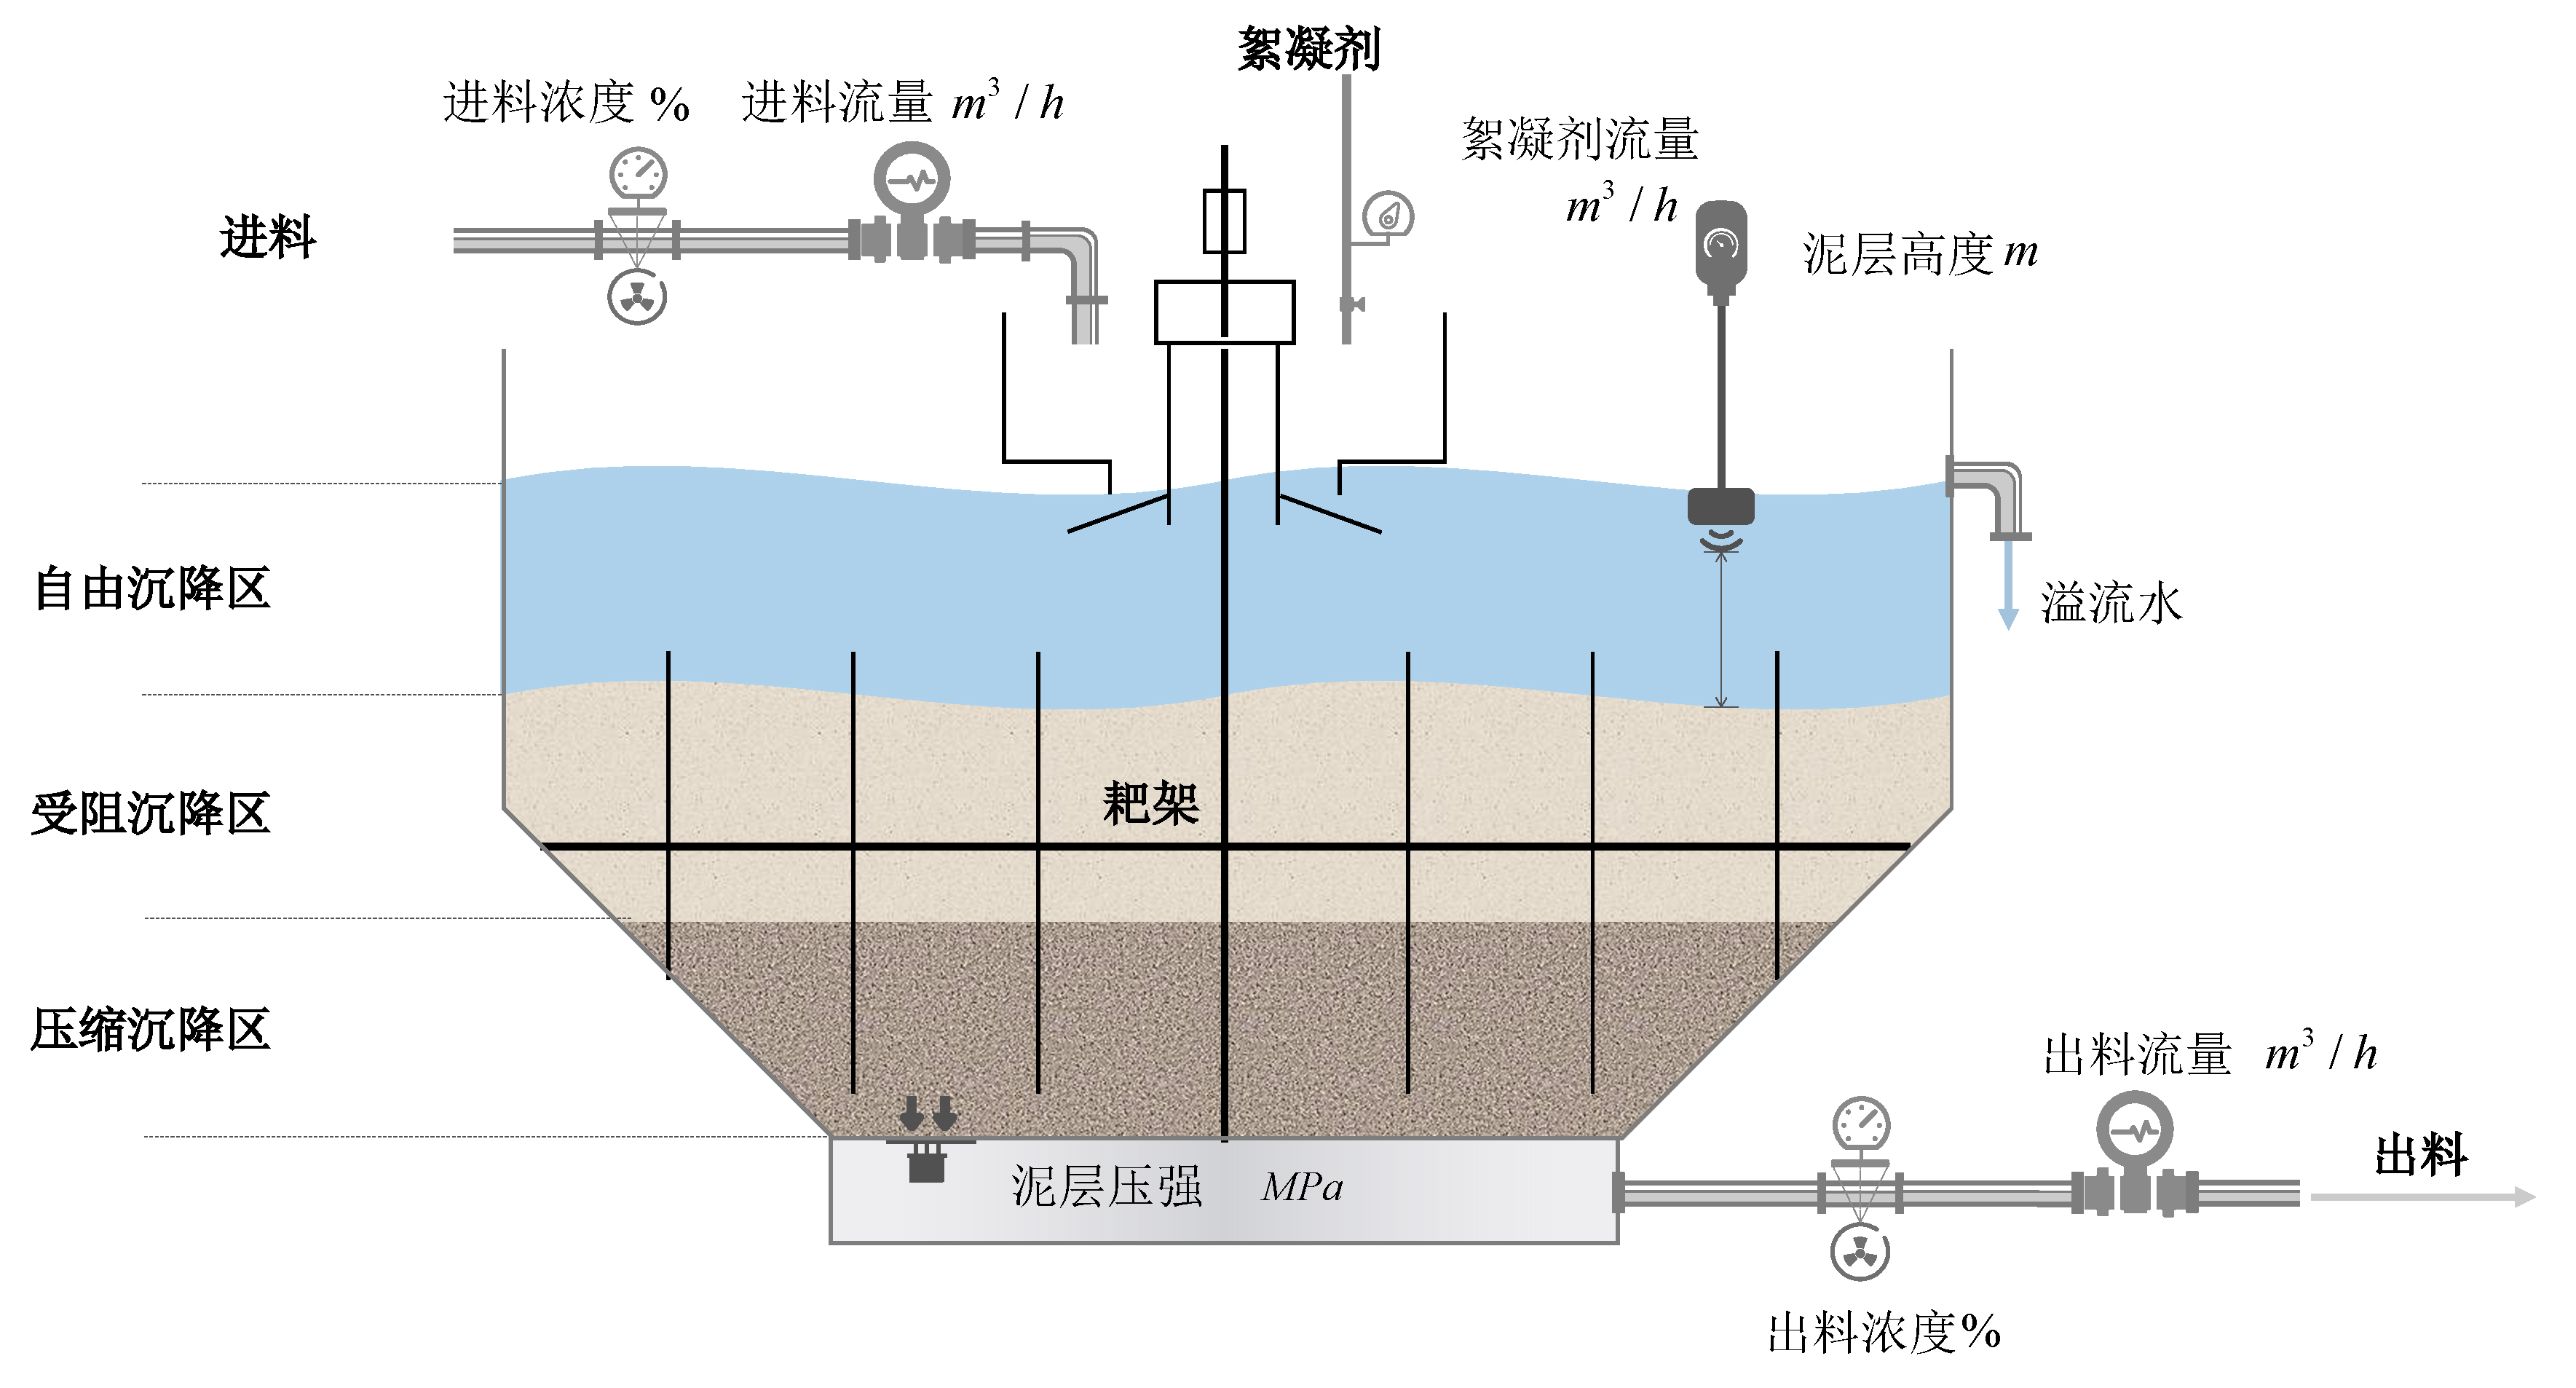
\includegraphics[width=\linewidth]{figures/chapter3/thickener.pdf}
\caption{
%%%%%%%%%%%%%%%%%%%%%%%%%%%
% seeking help: 如图所示,在实验的充填站,共有两台深锥浓密机,其中一主用,一备用,本文实验数据全部来源于第一台主用设备。
%As the figures illustrate above, there are two identical paste thickeners in the experimental backfilling station. One of them is primary device and the other is a spare. All of the original dataset in experiments are exported from the primary one.
膏体浓密机系统运行过程及监测变量图示
% The training data we use in this paper is collected from the primary device.
}
%%%%%%%%%%%%%%%%%%%%%%%%%%%
\label{fig:nfca_thickener}
%\vspace*{-0.3cm}
\end{figure}

% This section presents experimental results for the proposed method on the dataset of real thickening systems.
本节给出了所述方法在真实膏体浓密机系统数据集上的预测实验结果。
实验只要探究三个问题:

\textbf{问题1}:相比于直接采用离散时序预测模型,使用深度连续时间网络和高精度ODE求解器建模预测工业系统能否获得更优的效果?

\textbf{问题2}:在预测任务中使用平稳系统和非平稳系统的优缺点是什么?

\textbf{问题3}: 不同的插值方法和序列编码器的编码长度会如何影响所提出的CT模型的准确性?
本节中,我们将首先介绍数据集、模型超参数以及训练和测试参数的配置。然后给出详细的实验结果。

\subsection{膏体浓密机系统数据集}
\label{sec:paste_introduction}
在实验环节中,本章所用的工业系统数据来自于赞比亚铜带省,NFCA非洲矿业有限公司的膏体浓密机。
该设备由FLSmidth公司生产。
如图~\ref{fig:nfca_thickener}所示。该设备用于在膏体充填站将铜尾矿浓缩成高浓度料浆以用于充填膏体的制备。
两台设备都运行在闭环PID控制模式下。
% The dataset includes some key parameters in paste thickener which are listed in Table~\ref{tab:monitor_points}.
% \begin{table*}[htpb]
% \caption{Detailed monitoring point list in thickener system}
% \label{tab:monitor_points}
% \centering
% %% \tablesize{} %% You can specify the fontsize here, e.g., \tablesize{\footnotesize}. If commented out \small will be used.
% \begin{tabular}{cccc}
% \toprule
% \textbf{Name} & \textbf{Symbol} & \textbf{Unit}	& \textbf{Point description}\\
% \midrule
% 	Feed flow rate 	& $x^0$			& $m^3/h$ & Flow speed of the feed with low concentration \\
% 	Feed concentration 	& $x^1$			& $\%$ & Concentration of the Feed flow \\
% 	Mud Pressure	& $y^0$			& $MPa$ & Mud pressure at the bottom of the tank\\
% 	Rake speed & $x^2$ & rpm & Rotating speed of rake in thickener \\
% 	Flocculant flow rate	& $x^3$			& $m^3/h$ & Dosage of the flocculant\\
% 	Underflow rate	& $x^4$			& $m^3/h$ & Flow speed of the discharged underflow\\
% 	Underflow concentration	& $y^1$			& $\%$ & Concentration of the discharged underflow \\
% \bottomrule
% \end{tabular}
% \end{table*}
实验所用全部数据采集于2018年5月到2019年2月,采集间隔为两分钟。表~\ref{tab:dataset}展示了部分数据。
\begin{table*}[ht]
\small
\centering
\caption{膏体浓密机系统数据样例}
\label{tab:dataset}
\resizebox{0.9\linewidth}{!}{
\begin{tabular}{cccccccc}
\toprule
 采集时间      & \begin{tabular}[c]{@{}c@{}}进料 \\ 流量\end{tabular} & \begin{tabular}[c]{@{}c@{}}进料 \\ 浓度\end{tabular} & \begin{tabular}[c]{@{}c@{}}泥层 \\ 压力\end{tabular} & \begin{tabular}[c]{@{}c@{}}耙架 \\ 转速\end{tabular} & \begin{tabular}[c]{@{}c@{}}底流 \\ 流速\end{tabular} & \begin{tabular}[c]{@{}c@{}}底流 \\ 浓度\end{tabular} & \begin{tabular}[c]{@{}c@{}}絮凝剂\\ 流速\end{tabular} \\ \hline
2018/5/9 10:20  & 164.47                                                    & 16.47                                                         & 18.41                                                   & 500.58                                                                                                                                                  & 58.96                                                     & 59.72                                  &4.30                          \\
2018/5/9 10:22 &169.21                                                   & 15.51                                                         & 17.99                                                   & 500.16                                                                                                                                                  & 61.56                                                     & 58.88                                     &4.06                        \\ 
2018/5/9 10:24 & 141.78                                                    & 15.30                                                         & 16.41                                                   & 500.56                                                                                                                                                  & 59.97                                                     & 59.26                                   &4.06                          \\
2018/5/9 10:26 & 305.67                                                    & 25.31                                                         & 16.11                                                   & 500.99                                                                                                                                                  & 59.46                                                     & 58.77                                   &4.07                          \\
2018/5/9 10:28 & 328.70                                                    & 28.28                                                         & 16.43                                                   & 501.42                                                                                                                                                  & 59.68                                                     & 59.43                                   &4.43                          \\
2018/5/9 10:30 & 323.96                                                    & 25.90                                                         & 17.11                                                   & 501.56                                                                                                                                                  & 61.40                                                     & 60.09                                   &4.40                          \\
\bottomrule
\end{tabular}}
\end{table*}
收集的数据集来自于7个监测传感器,
系统输出变量$\b y(k) \in \mathbb{R}^2$中,包括底流浓度$y_1(k)$和泥层压力$y_2(k)$。
$y_1(k)$和$y_2(k)$均受到控制输入$\b x(k)\in \mathbb{R}^5$影响,包括进料流量$u_1(k)$、进料浓度$u_2(k)$、耙架转速$u_3(k)$、底流流量$u_4(k)$和絮凝剂流量$u_5(k)$。
删除系统停机时的异常监测数据,累计剩余24,673条数据。

本节采用滑动窗口法生成训练及测试样本对$(\b X _p^N, \b Y _p^N, \b X _f^M, \b Y _f^M)$,。
具体地,原始数据集依照浓密机系统的启停时间,分为多个文件。每个文件包含了连续生产过程中7个传感器的监测数据序列,且各序列中数据点的采样间隔均为2分钟。
对于每个文件中的多个序列,将大小为$N+M$的滑动窗口沿着序列的时间维度正向移动,移动步长为1。
% 为了从中的多个数据序列构建样本对$(\b X _p^N, \b Y _p^N, \b X _f^M, \b Y _f^M)$,
当窗口到达$i$位置时,四个序列$(\b X _p^N =\b X[i:i+N]$, $\b Y _p^N =\b Y[i:i+N]$, $\b X _f^M=\b X[i+N:i+N+M]$, $\b Y _f^M=\b Y[i+N:i+N+M])$被收集作为训练或测试样本。

%%%%%%%%%%%%%
% seeking help: 理想情况下,让滑动窗口的移动距离等于$N+M$ 是最佳的选择,这样可以保证任何两个训练数据对之间不存在交叉
%Ideally, it is the best choice that setting moving steps of sliding window equals to $N+M$ which keep no intersection of any two pieces.
% Ideally, it is the best choice to set the moving steps of the sliding window to $N+M$. This can guarantee that there is no intersection of any training data.
%%%%%%%%%%%%%
% However, when the total length of the original data from a thickening system is $|S|$, the remaining data groups count only $\frac{|S|}{N+M}$, which is not sufficient to train our complex model.
在验证集和测试集数据中,滑动窗口的大小设置为$N+L$,其中$L$表示待预测序列的长度(可能不等于训练集中待预测序列的长度$M$)。
模型仅通过训练集数据进行训练,然后使用不同的$L$在不同的验证集和测试集数据上进行验证和评估。
% The detailed parameters will be introduced in experimental paragraph.
% The detailed procedure for constructing datasets is illustrated in Fig.~\ref{fig:dataset}.
构造数据集的详细过程如图~\ref{fig:dataset}所示。
\begin{figure}[t]
    \centering
    %\vspace{-5pt}
    %\setlength{\abovecaptionskip}{-0.1cm} 
    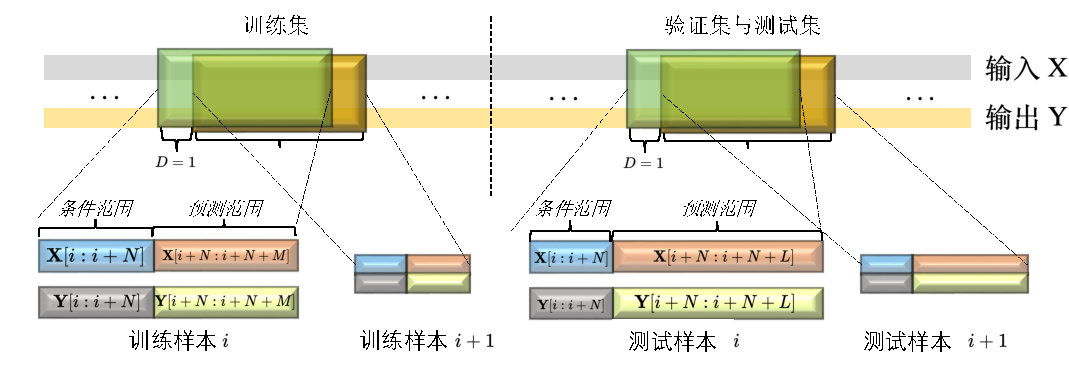
\includegraphics[width=\linewidth]{figures/chapter3/dataset.pdf}
    \caption{
    % Training set is built by moving a sliding window with speed $2$. Validation set and test set are built by moving a sliding window with speed $N+L$. $N$ is the length of encoded historical sequence. M is the length of predicted sequence in training phase. L is the length of predicted sequence in test or validation phase and it is a variable in different experiments.
    训练集、验证集、测试集的构建过程图示
    }
    \label{fig:dataset}
%\vspace*{-0.4cm}
\end{figure}

本节使用数据集的前$70\%$用于模型训练。在剩下的$30\%$中,前$15\%$作为验证集,帮助确定最佳训练轮次,剩下的$15\%$作为测试数据集用于评估模型准确性。
训练时,历史序列的长度为$N=80$,预测序列长度为$M=60$。
测试环节探究了$L=60, 200, 500$三种情况下,模型的预测性能。
根据图~\ref{fig:dataset}所示的构建输入-输出序列对的方法,共计17131个样本对用于训练。对于不同预测长度$L=60、200、500$,分别有3561、3421、3121个样本对用于测试和验证。
所有的数据在训练和测试之前均被归一化为标准正态分布。




\subsection{实验设定}

实验中,使用mini-batch随机梯度下降(SGD)和Adam优化器\cite{kingma2014adam}对模型进行训练。
batch size为$512$,学习速率为$0.001$,并且呈指数衰减。
衰减率为$0.95$,衰减周期为10个训练轮次。
ODE-net中隐藏状态$\b h(t)$的大小为$32$。
RNN序列编码器模块包含一个隐藏层,隐状态大小等于$32$,这隐状态$\boldsymbol h(t)$的大小一致。
状态解码器中隐藏层的大小为$64$。
在设定自适应微分方程求解器参数时,由于降低近似误差的容忍度,会导致求解常微分方程的时间剧烈增加。
在所有的实验中,为了平衡时间消耗和预测精度,我们将所有ODE求解器容忍的最大相对误差设置为$1\mathrm{e}-4$,容忍的最大绝对误差设置为$1\mathrm{e}-5$。
训练时,找到在验证集上预测精度最高的模型,将其用于测试数据集精度评估。
训练和测试均在单个Nvidia V100 GPU上进行。
代码基于PyTorch框架实现。
对于给定的离散整数下标序列$[0,1,\dots, M]$, 我们定义其连续时间区间为 $0\leq t\leq M\delta_t$.
相邻数据点的时间间隔$\delta _t$被设置为0.1。
因此,公式\eqref{equ:stationary}中的归一化因子$\mu _t$也被设置为0.1。
当使用欧拉数值求解器求解稳定系统的ODE方程时,模型将等价于使用GRU单元在离散时间系统下进行预测:
% \begin{equation}
\begin{align}
    \b h(t+\delta _t) &=\b h(t) + \delta _t \cdot \frac{\text{GRU}\big(\b h(t),x(t), \theta_d \big) - \b h(t)}{\mu _t}  \nonumber\\
                      &= \text{GRU}\big(\b h(t),x(t), \theta _d\big).
\end{align}
% \end{equation}

本节使用模型预测底流浓度的平均根相对平方误差(RRSE)和平均平方误差(MSE)评价不同模型的预测精度。
对于预测长度$L$,RRSE定义如下:
\begin{equation}
\begin{aligned}
    \text{RRSE}=\sqrt{\sum_{j=1}^{L} \frac{e_{j}^{2}}{\left(\hat{y}_{j}-\bar{y}\right)^{2}}}, \quad e_{j}=\hat{y}_{j}-y_{j}.
\end{aligned}
\label{equ:rrse}
\end{equation}
RRSE可以解释为被归一化的均方根(RMS)误差。

% \subsection{实验结果分析与讨论}

% To demonstrate the significance of proposed continuous-time system identification model.
% We construct two kinds of competitive baselines for substituting derivative module:
% \begin{equation}
%     \label{equ:nodiff_rnn}
%     \boldsymbol{h}(i+1)=R(\boldsymbol{h}(i), \boldsymbol{x}(i))
% \end{equation}
% \begin{equation}
%     \label{equ:diff_rnn}
%     \boldsymbol{h}(i+1)=R(\boldsymbol{h}(i), \boldsymbol{x}(i)) + \epsilon \boldsymbol{h}(i)
% \end{equation}
% Model with structure \eqref{equ:nodiff_rnn} is basic recurrent neural networks model which can be used to learn time series model and stationary system.

\subsection{不同模型预测结果对比}
首先,我们研究了不同ODE求解器和导数模块对预测精度的影响。
我们选择了四个ODE求解器:Euler, midpoint,四阶Runge—Kutta (RK4), Dormand—Prince (Dopri5)\cite{NIPS2018_7892},以及三阶Bogacki—Shampine(Bosh)\cite{bogacki19893}。我们研究了这些微分方程求解器结合非稳定和稳定系统时的性能。
此外,我们还对比了离散时间深度序列模型,包括状态空间(DT-State-Space)、基于注意力机制的Seq2Seq模型(Attention-Seq2Seq)\cite{Member2019}和Transformer模型\cite{Wu2020}。
DT-State-Space~\cite{Rangapuram2018}模型采用循环神经网络(RNN)建模线性状态空间模型的参数,并基于预测得到的状态空间模型预测时间序列。其状态空间和RNN隐藏层的大小分别设置为16和32。
Transformer和Attention-Seq2Seq的超参数设置与原文献保持一致。

我们进行了三组实验以探究不同预测长度$L=60$、$200$和$500$下,不同模型预测结果的RRSE、MSE和预测速度。
% Table~\ref{tab:exp_all} presents the results of the predicted underflow concentrations. 
\begin{table*}[htpb]
%\setlength{\abovecaptionskip}{-0.1cm} 
\caption{
%%%%%%%
% seeking help : 预测底流浓度的RRSE、MSE 误差 以及每次预测序列所需的时间
%RRSE and MSE error of predicted underflow concentration and time consumption for each prediction.
Root relative squared error (RRSE), mean squared error (MSE), and time consumption of predicted underflow concentration.
}
%%%%%%%
\label{tab:exp_all}
\centering
% \setlength{\tabcolsep}{3.0mm}{%7可随机设置,调整到适合自己的大小为止
\resizebox{\linewidth}{!}{
\footnotesize
\renewcommand{\arraystretch}{1.5}
\begin{tabular}{c|c|ccccccccc}
\toprule
\multicolumn{2}{c|}{\multirow{2}{*}{模型}}                                                                        & \multicolumn{3}{c|}{$L=60$}                                                           & \multicolumn{3}{c|}{$L=200$}                                                           & \multicolumn{3}{c}{$L=500$}                                         \\ \cline{3-11} 
\multicolumn{2}{c|}{}                                                                                              & RRSE                 & MSE                  & \multicolumn{1}{c|}{Time (s)}             & RRSE                 & MSE                  & \multicolumn{1}{c|}{Time (s)}              & RRSE                 & MSE                  & Time (s)                \\ \hline
\multirow{4}{*}{\begin{tabular}[c]{@{}c@{}}非稳定\\ 系统\end{tabular}} & \multicolumn{1}{c|}{Euler}     & 3.18                 & 9.07                 & \multicolumn{1}{c|}{1.71}             & 5.09                 & 80.25                & \multicolumn{1}{c|}{3.81}              & 3.95                 & 152.21               & 4.65                 \\
                                                                                 & \multicolumn{1}{c|}{Mid-Point} & 3.10                 & 8.95                 & \multicolumn{1}{c|}{3.23}             & 5.24                 & 80.29                & \multicolumn{1}{c|}{7.36}              & 4.16                 & 172.43               & 9.15                 \\
                                                                                 & \multicolumn{1}{c|}{RK4}       & 3.10                 & 8.97                 & \multicolumn{1}{c|}{6.95}             & 5.24                 & 83.90                & \multicolumn{1}{c|}{14.82}             & 4.16                 & 172.64               & 18.76                \\
                                                                                 & \multicolumn{1}{c|}{Bosh}    & 3.08  & 8.57  & \multicolumn{1}{c|}{12.8}             & 5.84                 & 84.60                & \multicolumn{1}{c|}{19.0}              & 4.61                 & 172.39               & 24.75                \\
                                                                                 & \multicolumn{1}{c|}{Dopri5}    &  \uline{\textbf{2.83}}  &  \uline{\textbf{6.40}}  & \multicolumn{1}{c|}{9.63}             & 5.31                 & 84.60                & \multicolumn{1}{c|}{13.8}              & 4.19                 & 175.39               & 25.75                \\ \hline
\multirow{4}{*}{\begin{tabular}[c]{@{}c@{}}稳定\\ 系统\end{tabular}}     & \multicolumn{1}{c|}{Euler}     & 3.18                 & 9.06                 & \multicolumn{1}{c|}{1.63}             & 3.75                 & 34.78                & \multicolumn{1}{c|}{3.58}              & 1.63                 & 37.77                & 4.66                 \\
                                                                                 & \multicolumn{1}{c|}{Mid-Point} & 3.18                 & 9.08                 & \multicolumn{1}{c|}{3.22}             & 3.73                 & 34.64                & \multicolumn{1}{c|}{7.17}              & 1.62                 & 38.36                & 9.3                  \\
                                                                                 & \multicolumn{1}{c|}{RK4}       & 3.18                 & 8.96                 & \multicolumn{1}{c|}{6.80}             &  \uline{\textbf{3.58}}  &  \uline{\textbf{32.90}} & \multicolumn{1}{c|}{15.17}             &  \uline{\textbf{1.61}}  &  \uline{\textbf{34.88}} & 18.66                \\
                                                                                 & \multicolumn{1}{c|}{Bosh}    & N/A                    & N/A                    & \multicolumn{1}{c|}{\textgreater{}50} & N/A                    & N/A                    & \multicolumn{1}{c|}{\textgreater{}200} & N/A                    & N/A                    & \textgreater{}3000   \\
                                                                                 & \multicolumn{1}{c|}{Dopri5}    & N/A                    & N/A                    & \multicolumn{1}{c|}{\textgreater{}50} & N/A                    & N/A                    & \multicolumn{1}{c|}{\textgreater{}200} & N/A                    & N/A                    & \textgreater{}3000   \\ \hline
\multicolumn{2}{c|}{Attention-Seq2Seq\cite{Member2019}}                                                                             & 3.13                 & 8.97                 & \multicolumn{1}{c|}{0.41}             & 4.02                 & 33.90                & \multicolumn{1}{c|}{0.41}              & 1.82                 & 40.53                & 0.42                 \\ \hline
\multicolumn{2}{c|}{DT-State-Space\cite{Rangapuram2018}}                                                                               & 3.22                 & 9.36                 & \multicolumn{1}{c|}{0.06}             & 4.69                 & 41.11                & \multicolumn{1}{c|}{0.07}              & 3.35                 & 45.64                & 0.08                 \\
\multicolumn{2}{c|}{Transformer\cite{Wu2020}}                                                                               & 3.16                 & 8.36                 & \multicolumn{1}{c|}{0.02}             & 3.99                 & 40.23                & \multicolumn{1}{c|}{0.02}              & 2.55                 & 44.23                & 0.03                 \\
\bottomrule
\end{tabular}}
\end{table*}

在表~\ref{tab:exp_all}中可以发现,离散时间域下的Attention-Seq2Seq模型、DT-State-Space模型和Transformer的性能稍优于使用Euler求解器的模型效果,但差于使用高阶ODE求解器获得的预测效果,特别是在长期预测$L=200, 500$时表现更为明显。
结果表明,采用连续时间模型可以更好地反映浓密机系统的连续时间演化特征,从而相比于纯离散时间模型,呈现更高的预测精度。

\subsection{不同ODE求解器对比}
进一步地,我们分别对采用了不同ODE求解器的稳定系统模型和非稳定系统模型进行分析比较。

当导数模块被定义为非稳定系统时,对于短期预测任务$L = 60$,
我们发现,虽然Euler求解器的时间消耗低于其他ODE求解器,但其预测结果的RRSE和MSE指标较高,预测精度差于使用其他四个ODE求解器。
原因在于欧拉方法作为求解ODE方程最简单的方法,它在两个相邻时间点之间仅仅调用导数模块计算隐状态的一阶导数一次,然后计算状态差分。其运行本质等同于离散时间序列模型,算得ODE方程的解的精度较差,并没有充分利用模型为连续时间系统的性质。
相应地,中值法和4阶Runge-Kutta法在两个相邻时间点之间,分别调用了导数模块计算隐状态导数2次和4次。因此,其对隐状态轨迹的求解精度高于欧拉法。
该结果也证实了,基于Euler方法的离散时间序列模型忽略了系统的连续时间特性,因此不能精确地学习系统的动态过程。
进一步地,作为隶属于龙格-库塔体系中的常微分方程自适应步长求解方法,Dopri5和Bosh方法能够确保数值近似解与真实解之间的误差限定在指定误差范围内。
随着给定误差限的缩小,求解ODE方程的时间消耗也随之增加。
虽然两种方法求解ODE耗时较长,但精度较高。Dopri5的预测性能稍好于Bosh。

%It is also equivalent to standard discrete-time deep sequential model which is the most common choice for formulating an evenly sampled dynamical system.

% 当导数模块分别被定义为非稳定系统与稳定系统时,ODE求解器在预测精度和时间消耗上表现也会收到
% 实验中,我们还发现,同一ODE求解器在预测精度和时间消耗上表现也会受到导数模块定义的影响。
当导数模块定义为平稳系统时。
两种自适应方法Bosh和Dopri5求解ODE方程的时间消耗将显著增加。
在表\ref{tab:exp_all}中,我们没有列出Dopri5和Bosh在稳定系统中的预测精度,因为其计算速度极慢,使得该方法不适用于实际工业应用。
对比其他ODE求解器,我们发现RK4等高阶ODE求解器的求解误差小于低阶ODE求解器,但在求解ODE方程时需要消耗更多的时间。


%are relatively higher order ODE solvers which have higher accuracy than Euler and evaluate the derivative network for 2 times and 4 times respectively between two adjacent time points. As an adaptive method in Runge–Kutta family, Dopri5 ensures that the output is within a given tolerance of true solution.
% while the decrease of tolerance is accompanied by the increases of times for evaluating the differential equation.
%%%%%%%%%%%%%%%%
% seeking help: 在Dopri5中,求解ODE的时间会伴随着减少误差容许度而增加,我们在实验中将相对容许度设置为1e-4, 绝对容许度设置为1e-5.
%In Dopri5, the time for evaluating the differential equation will increase if we reduce the tolerance of calculation error. 
%In all of experiments, we set the relative tolerance to $1e-4$ and absolute tolerance to $1e-5$.

% According to our industrial requirement from the system, we set the relative tolerance to $1e-4$ and absolute tolerance to $1e-5$.

%%%%%%%%%%%%%%%%
% The definition of $RNN$ in \eqref{equ:non_stationary} and \eqref{equ:stationary} varies from basic RNN to GRU, ASRNN and and simple (Multi-Layer Perceptron, MLP).


% The form \eqref{equ:diff_rnn} adds a skip connection based on original RNN which can be interpreted as Euler approximation of ODE-net model. 
% $epsilon$, an experimental parameter, is set to $0.1$ to restrain the fluctuation of hidden state.
% Under the assumption of continuous-time property in thickening system, form \eqref{equ:diff_rnn} is considered to perform better than \eqref{equ:nodiff_rnn} in theory.
% In our experiment, RNN, LSTM, GRU, ASRNN are original sequential models with structure \eqref{equ:nodiff_rnn}, 
% and the identifiers RNN-Diff, LSTM-Diff, GRU-Diff, ASRNN-Diff represent the networks with skip connection \eqref{equ:diff_rnn}. 
% These discrete-time models depends on the data are sampled evenly which is satisfied in our experiment, 

% A closer model with ODE-net is Runge-Kutta neural network~\cite{Wang1998} which is a approximation of continuous-time model.
% We set the order of Runge-Kutta network as 4 and the output is described by:
% A thorough experiment in Tab.\ref{tab:exp_all} is conducted to study the influence from ODE solver and system dynamic to prediction accuracy and time cost. 
% In Tab.\ref{tab:exp_all}, only the metrics on underflow concentration are listed in the table because underflow concentration is generally more noteworthy than mud pressure in thickening system.
%For the experiments with $L=60$ as shown in Table~\ref{tab:exp_all}, the length of predicted sequence is relatively shorter than other experimental groups.


% \paragraph{Comparison of stationary models and non-stationary models}
\subsection{稳定系统与非稳定系统对比}

为了更直观地比较使用稳定系统和非平稳系统定义导数模块的区别,我们进一步地可视化了不同ODE求解器对非稳定和稳定系统的预测效果。
图\ref{fig:predict_cmp_60}描述了对于$L=60$的短期预测任务,使用不同ODE求解器求解非平稳系统和平稳系统得到的预测序列:
\begin{figure}[h]
\centering
%\setlength{\abovecaptionskip}{-0.1cm} 
\subfigure[稳定系统+RK4求解器]{
\begin{minipage}[t]{0.33\linewidth}
\centering
% \hspace{-22pt}
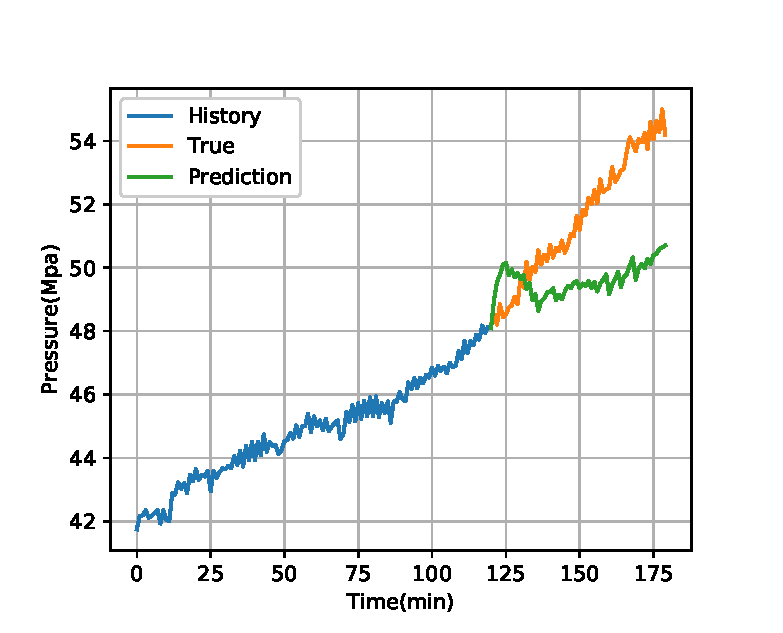
\includegraphics[width=\linewidth,trim=12 0 0 20,clip]{figures/chapter3/predict_cmp/Pressure_GRU_sta_rk4_60.eps}
% \hspace{-18pt}

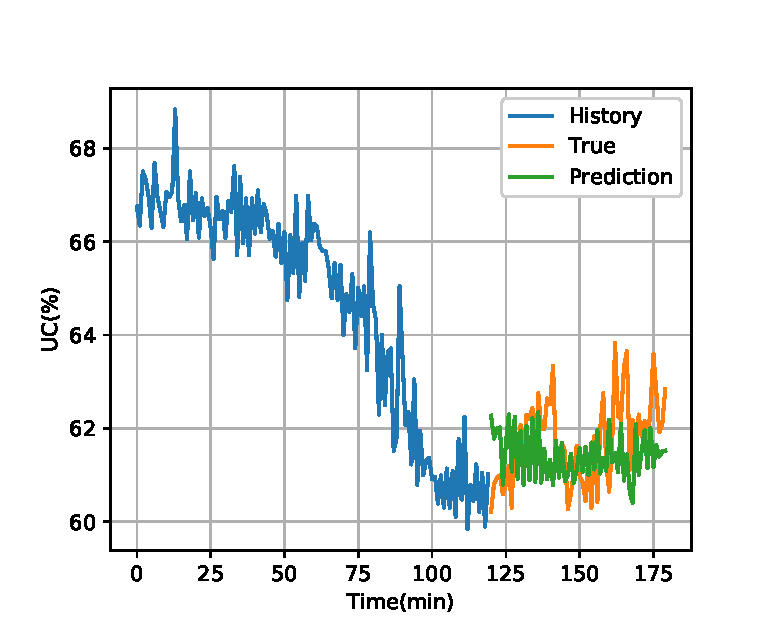
\includegraphics[width=\linewidth,trim=12 0 0 20,clip]{figures/chapter3/predict_cmp/UC_GRU_sta_rk4_60.eps}
%\caption{fig1}
\end{minipage}
}%
\hspace{-22pt}
\subfigure[非稳定系统+RK4求解器]{
\begin{minipage}[t]{0.33\linewidth}
\centering
% \hspace{-22pt}
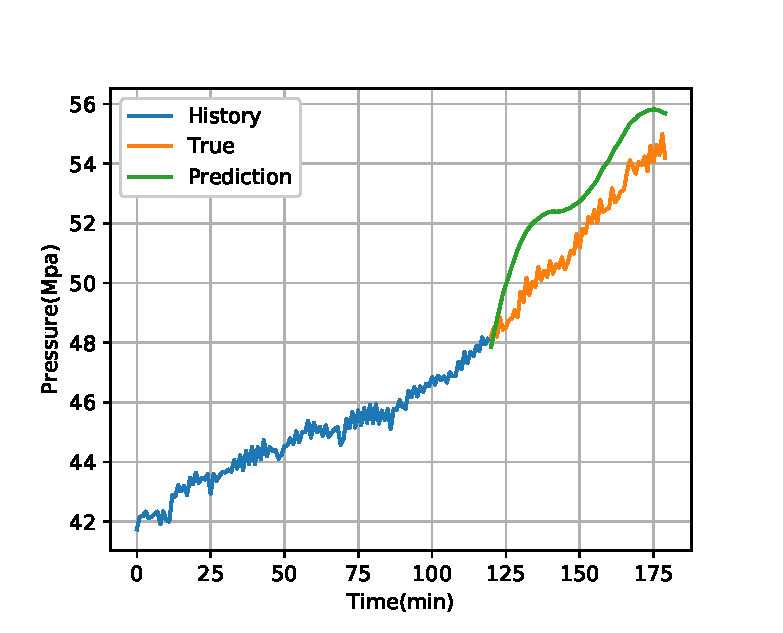
\includegraphics[width=\linewidth,trim=12 0 0 20,clip]{figures/chapter3/predict_cmp/Pressure_MLP_nonsta_rk4_60.eps}
% \hspace{-18pt}

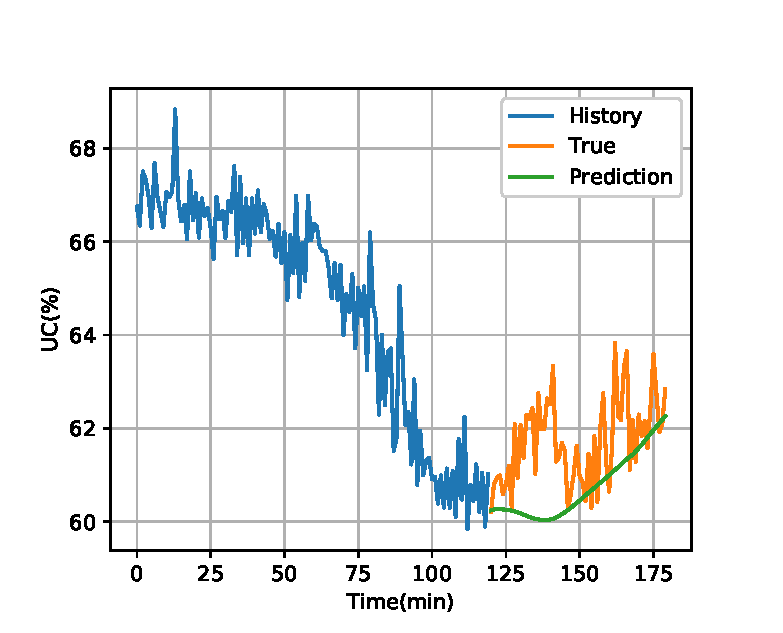
\includegraphics[width=\linewidth,trim=12 0 0 20,clip]{figures/chapter3/predict_cmp/UC_MLP_nonsta_rk4_60.eps}
%\caption{fig1}
\end{minipage}
}%
\hspace{-22pt}
\subfigure[非稳定系统+Dopri5求解器]{
\begin{minipage}[t]{0.33\linewidth}
\centering
% \hspace{-22pt}
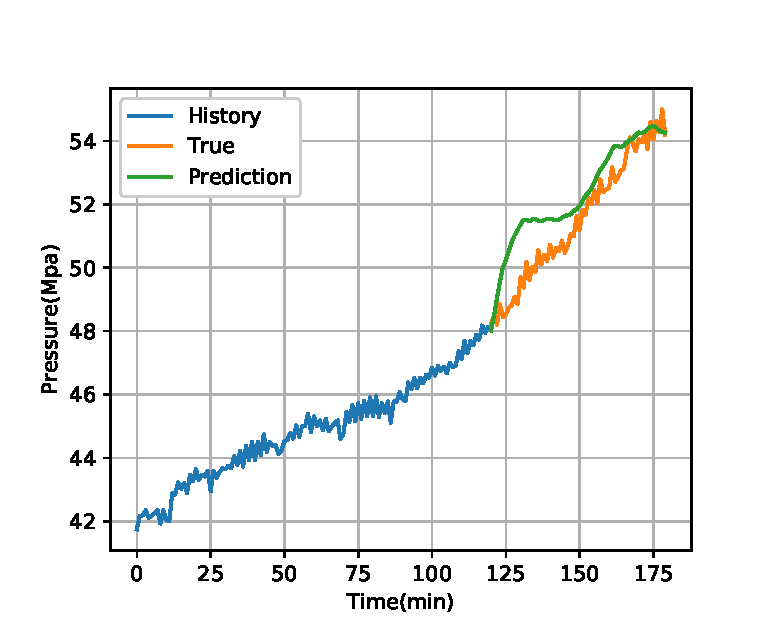
\includegraphics[width=\linewidth,trim=12 0 0 20,clip]{figures/chapter3/predict_cmp/Pressure_MLP_nonsta_dopri5_60.eps}
% \hspace{-18pt}

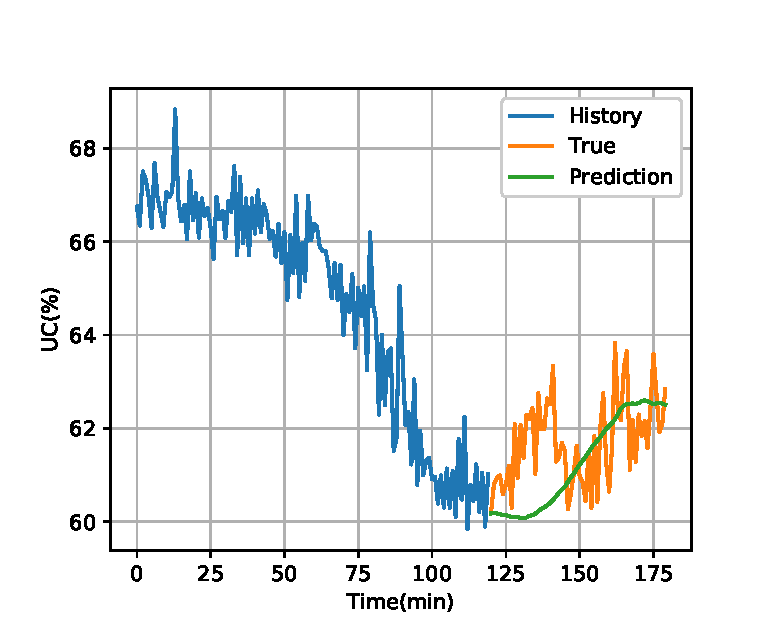
\includegraphics[width=\linewidth,trim=12 0 0 20,clip]{figures/chapter3/predict_cmp/UC_MLP_nonsta_dopri5_60.eps}
%\caption{fig1}
\end{minipage}
}%
\centering
\caption{不同系统及不同ODE求解器在$L=60$短期预测任务中的性能比较}
\label{fig:predict_cmp_60}
%\vspace*{-0.4cm}
\end{figure}

结果表明,非平稳模型在短期预测任务中的表现优于平稳模型。非平稳模型的估计序列比平稳模型的估计序列更接近实际系统输出。
非平稳系统的学习过程本质上相当于对隐状态进行差分,利用MLP网络学习平稳的系统一阶差分。
% The non-stationary system learns the evolution of internal hidden state which 
% The model with non-stationary system dynamic identifies the system smoothly because the structures constraint hidden state can only change in a continuous and slow form.
% TODO: 真的不想删,但是受篇幅限制暂时注释,以后有机会偷偷补上
此外,由于非稳定系统结构限制了隐状态只能以连续、缓慢的方式变化。因此模型可以平滑地预测系统的输出。该约束符合浓密机系统运行缓慢的特性,等价于缩小了模型参数的搜索空间,抑制了模型过拟合的情况。

图\ref{fig:predict_cmp_200}展示了长期预测任务($L=200$)中的模型预测结果。
% ($L=500$的类似结果可以在Table~\ref{tab:exp_all}中找到)。
\begin{figure}[t]
%\setlength{\abovecaptionskip}{-0.1cm} 
\centering
\subfigure[非稳定系统+RK4求解器]{
\begin{minipage}[t]{0.33\linewidth}
\centering
% \hspace{-22pt}
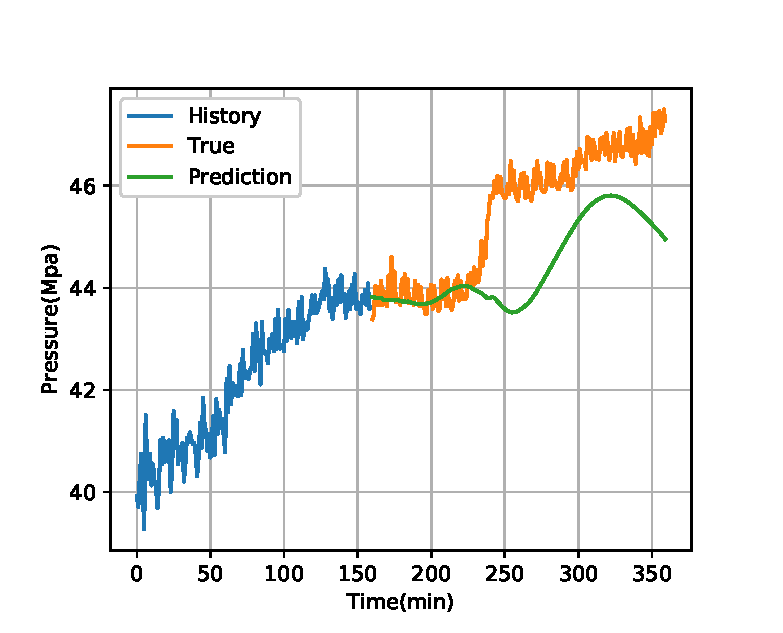
\includegraphics[width=\linewidth,trim=12 0 0 20,clip]{figures/chapter3/predict_cmp/Pressure_MLP_nonsta_rk4_200.eps}
% \hspace{-18pt}

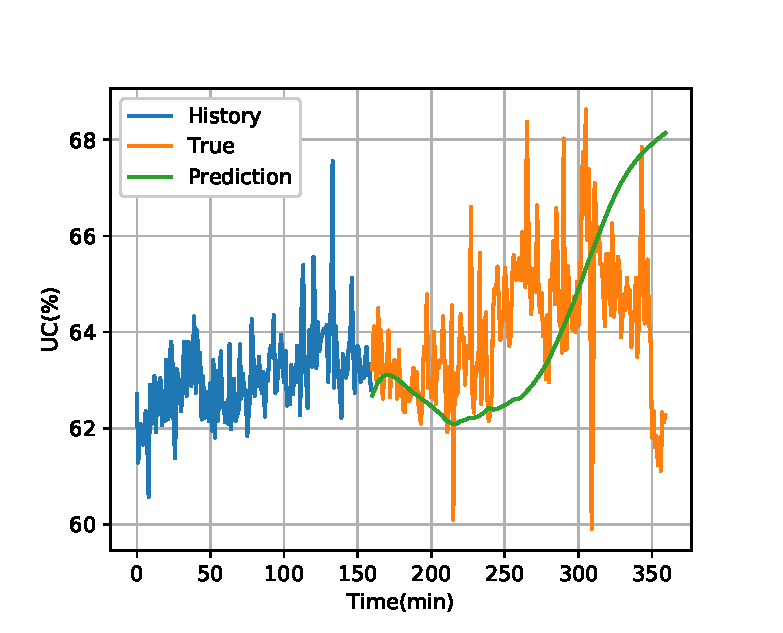
\includegraphics[width=\linewidth,trim=12 0 0 20,clip]{figures/chapter3/predict_cmp/UC_MLP_nonsta_rk4_200.eps}
%\caption{fig:subfig_200_nonsta_rk4}
\end{minipage}
\label{fig:subfig_200_nonsta_rk4}
}%
\hspace{-22pt}
\subfigure[稳定系统+Euler求解器]{
\begin{minipage}[t]{0.33\linewidth}
\centering
% \hspace{-22pt}
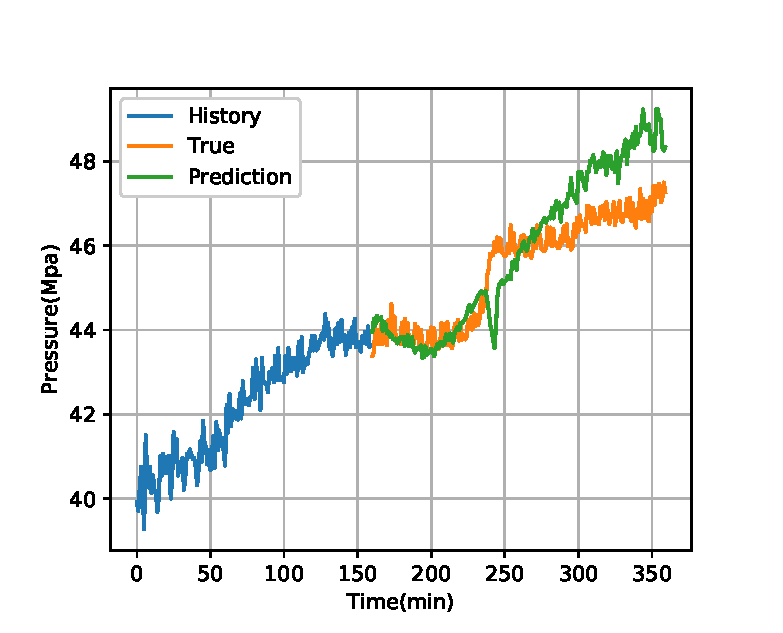
\includegraphics[width=\linewidth,trim=12 0 0 20,clip]{figures/chapter3/predict_cmp/Pressure_GRU_sta_euler_200.eps}
% \hspace{-18pt}

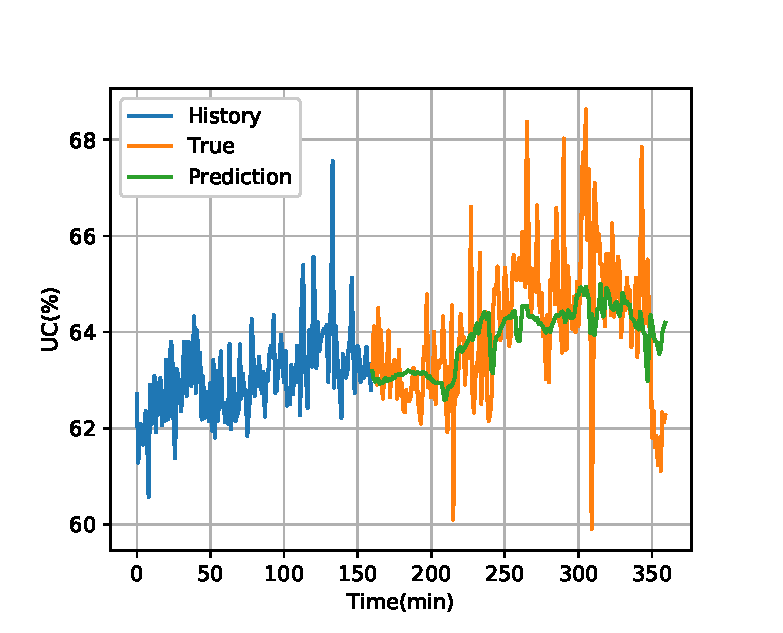
\includegraphics[width=\linewidth,trim=12 0 0 20,clip]{figures/chapter3/predict_cmp/UC_GRU_sta_euler_200.eps}
%\caption{fig:subfig_200_sta_euler}
\end{minipage}%
\label{fig:subfig_200_sta_euler}
}%
\hspace{-22pt}
\subfigure[稳定系统+RK4求解器]{
\begin{minipage}[t]{0.33\linewidth}
\centering
% \hspace{-22pt}
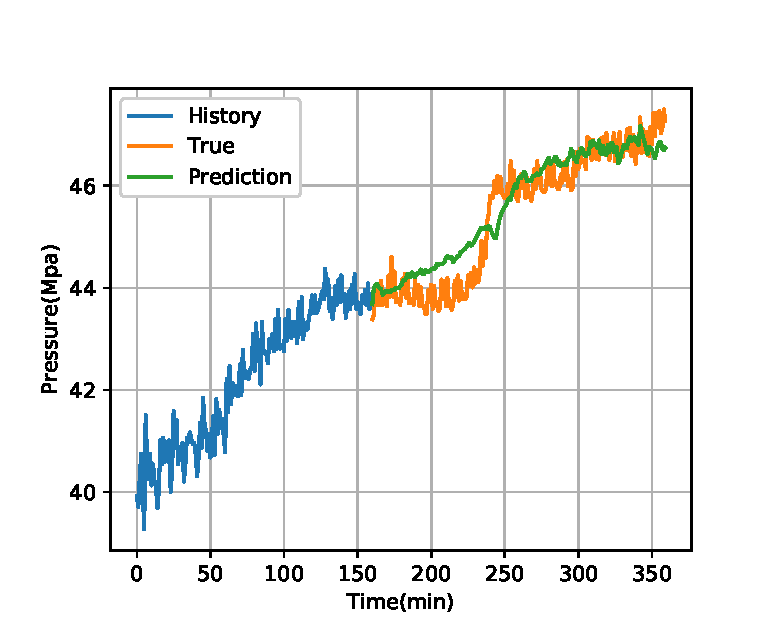
\includegraphics[width=\linewidth,trim=12 0 0 20,clip]{figures/chapter3/predict_cmp/Pressure_GRU_sta_rk4_200.eps}

% \hspace{-18pt}
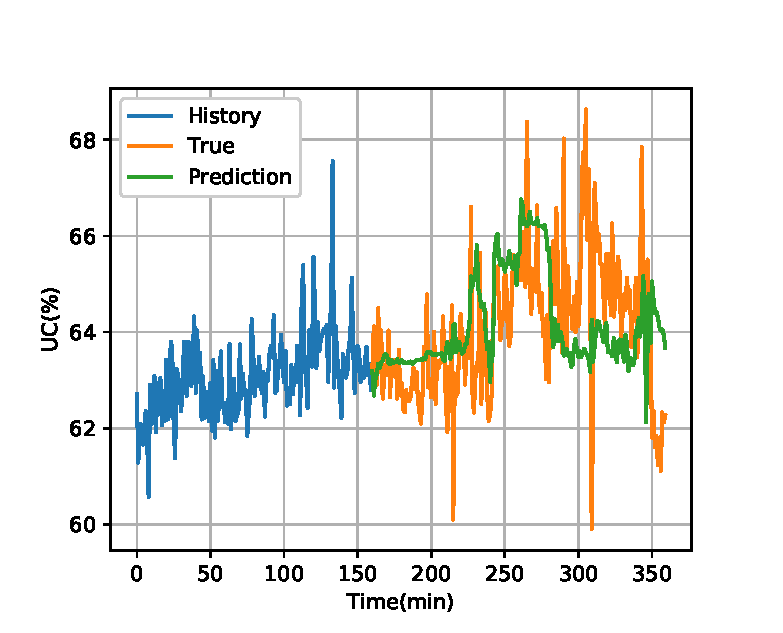
\includegraphics[width=\linewidth,trim=12 0 0 20,clip]{figures/chapter3/predict_cmp/UC_GRU_sta_rk4_200.eps}
%\caption{fig:subfig_200_sta_rk4}
\end{minipage}%
\label{fig:subfig_200_sta_rk4}
}%
% \subfigure[RNN-sta-Euler]{
% \begin{minipage}[t]{0.31\linewidth}
% \centering
% \includegraphics[width=1.1\linewidth]{figures/chapter3/predict_cmp/UC_RNN_sta_euler_200.eps}
% %\caption{fig2}
% \end{minipage}
% }%
\centering
\caption{$L=200$时,不同ODE求解器、系统动态的预测效果对比
} 
\label{fig:predict_cmp_200}
%\vspace*{-0.3cm}
\end{figure}
图中呈现的预测效果与表\ref{tab:exp_all}中的结果几乎一致。在长期预测任务中,非平稳模型的RRSE和MSE远远高于平稳模型,模型预测效果更差。
%It is meaningless to compare RRSE indices of results with different $L$, despite the RRSE in the experiments with $L=500$ is lower than $L=200$.
% When , we find that the model with stationary system performs lower prediction error than the non-stationary method.
% The illustrations of predicted results shown in Fig. \ref{fig:predict_cmp_200} and Fig. \ref{fig:predict_cmp_500} demonstrate that the non-stationary model only performs well in early period.
% The illustrations of predicted results shown in Fig. \ref{fig:predict_cmp_200} demonstrates that the non-stationary model only performs well in early period.
% We also illustrate the predicted results with $L=200$ in Fig. .
从图\ref{fig:predict_cmp_60}可以看出,非平稳模型在短期预测问题中获得较好的预测效果。
而在图\ref{fig:subfig_200_nonsta_rk4}中,非稳定系统在长期预测场景下的预测精度显著衰减,且预测偏离程度伴随着预测序列长度的增加而增加。
与之相对地,稳定系统的预测结果是稳定的,更接近于系统的真实输出,这证明了稳定系统模型在长期预测问题中具有更好的准确性。
% It is meaningless to compare RRSE indices of results with different $L$.
在由非稳定系统定义的导数模块中,其内部结构导致了隐状态在积分过程中是无约束的,状态的取值空间将逐渐扩张。
虽然模型在解码器网络中嵌入$\tanh$函数,能够将预测的系统输出限制在合理的范围内,但解码器模块无法学习有效的映射函数,实现从极大的隐状态空间到系统输出空间的准确映射。

同样地,图~\ref{Fig:predict_cmp_200}也证明了在长期预测问题中,高阶ODE求解器(如4阶Runge—Kutta)能够获得比低阶ODE求解器(如Euler)更好的预测效果。


% It notes that in the last part of simulation, the predicted system outputs deviate from the real sequences.
% The error is produced because thickening system is a partially observed system.
% Except for known external input or interference in $\b x(t)$, there exist plenty of invisible disturbances which affect the system extremely.
% The negative effects from unknown disturbances make the errors accumulated continuously over a long time period.
% In the long-term prediction task with $L=500$, the stationary model predicts the system outputs well in the former 300 minutes.




% TODO: 这部分也暂时注释,日后有机会再补上
%%%%%%%%%
% seek help: 自回归模型的缺点也是很明显的,每一轮循环的推理必须要在上一轮计算完成之后才能开始,ODE-net也不例外
% The disadvantage of autogressive model is also obvious that, each round of recurrent inference has to done after the last round finished, and ode-net is no exception.
% One disadvantage for autoregressive model is the recurrent inference must follow by rounds, so does ODE-net.
%%%%%%%%%

% 结果证实了基本rnn由于忽略了增稠系统的连续时间特性而不能很好地学习系统动力学方程的猜测。

从实验结果可以看出,采用自适应求解器的连续时间ODE-Net的预测表现优于其他欧拉近似法和龙格库塔近似法。
说明微分方程求解的精度会严重影响模型预测的精度。

虽然本文所提出的连续时间ODE-Net模型在预测精度上表现良好,但与其他模型相比,推理速度较慢。
表\ref{tab:exp_all}的最后一列表示预测序列长为$L$时,模型的平均消耗时间。
因为在ODE-net的训练和推理中,其前向传播和反向传播过程都需要大量地计算隐状态导数。
因此在预测系统动态变化时,其时间消耗远高于离散时间模型。
一些前沿研究\cite{J2020,poli2020,kelly2020}聚焦于优化ODE-net的训练或推理速度。
这些方法为提高本文模型的预测效率提供了有借鉴意义的指导。


本节额外进行了数组实验,以评估在不同预测长度$L$下,稳定系统和非稳定系统预测的底流浓度误差(MSE)变化。
图~\ref{fig:length_cmp}展示了五次重复实验中,底流浓度的预测误差波动情况($ log_{10}{\text{MSE}} \pm 2\sigma$)。虽然在长期预测任务中稳定系统优于非稳定系统,但非稳定系统在短期预测任务中的表现优于稳定系统(如$L<100$)。
大约当$L$超过$120$时,非稳定系统的误差随预测长度的增加而显著增加。
\begin{figure}[htpb]
%\setlength{\abovecaptionskip}{-0.1cm} 
    \centering
    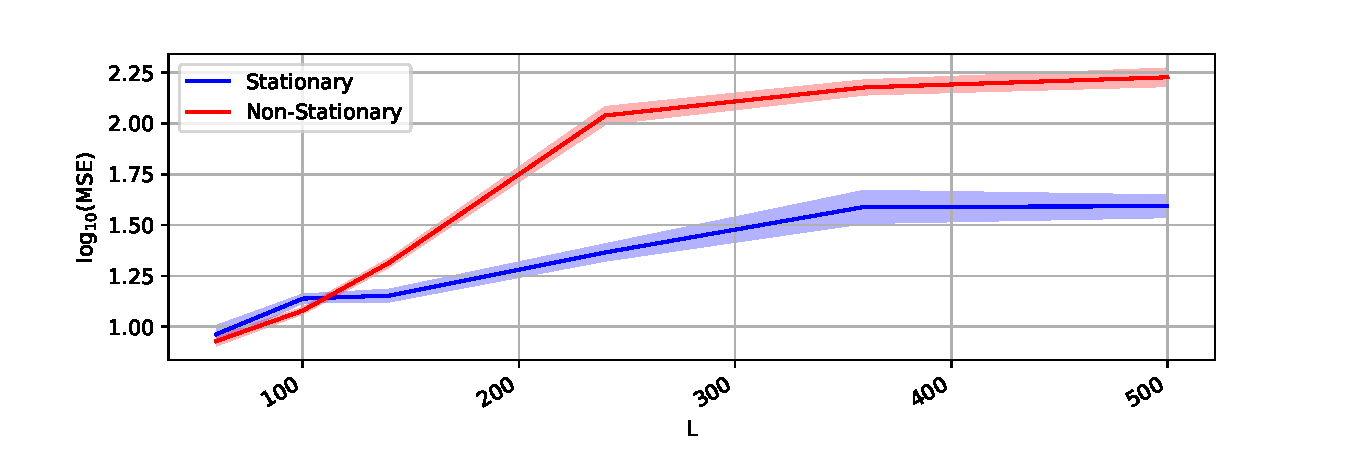
\includegraphics[width=\linewidth,trim=50 0 50 10, clip]{figures/chapter3/length_cmp.pdf}
    \caption{
    % The predicted length $L$ affects average $\log_{10}{MSE} \pm 2\sigma$ range of predicted underflow concentration for both stationary and non-stationary system.
    不同预测长度下稳定系统和非稳定系统的预测精度变化
    }
    \label{fig:length_cmp}
%\vspace*{-0.4cm}
\end{figure}

\subsection{探究序列插值阶数的对预测精度的影响}
本小节将进行消融实验,以探究对离散输入序列进行插值的方法是否对预测精度产生影响。
我们测试了四种不同阶数的样条插值方法,并比较了模型在测试集上的预测精度。
% The recurrent cell in experiment is RNN and the schema for solving ODE is RK4 uniformly.
表~\ref{tab:interolopation_cmp}的结果表明,模型中采用高阶插值的精度将稍优于低阶插值。
\begin{table}[h]
\centering
%\setlength{\abovecaptionskip}{-0.1cm} 
\caption{不同插值方法对预测精度的影响}
\renewcommand{\arraystretch}{1.5}
\label{tab:interolopation_cmp}
\begin{tabular}{c|cc|cc|cc}
\toprule
 \multirow{2}{*}{模型}         & \multicolumn{2}{c|}{\begin{tabular}[c]{@{}c@{}}$L=60$ \\ (120 minutes)\end{tabular}}                 & \multicolumn{2}{c|}{\begin{tabular}[c]{@{}c@{}}$L=200$ \\ (400 minutes)\end{tabular}}                  & \multicolumn{2}{c}{\begin{tabular}[c]{@{}c@{}}$L=500$ \\ (1000 minutes)\end{tabular}}                 \\
    & RRSE                 & MSE                  & RRSE                 & MSE                   & RRSE                 & MSE                   \\ \hline
三次样条插值     &  \uline{\textbf{3.083}} & \uline{ \textbf{8.565}} & \uline{ \textbf{3.581}} & 32.90                & 1.615                & \uline{\textbf{ 34.88}} \\
二次样条插值 & 3.097                & 8.993                & 3.593                &\uline{ \textbf{32.585}} &\uline{ \textbf{1.613}} & 36.741                \\
线性插值   & 3.098                & 8.999                & 3.763                & 33.530                & 1.627                & 37.778                \\
零阶样条插值      & 3.115                & 9.050                & 3.791                & 33.585                & 1.628                & 37.695                \\ \bottomrule
\end{tabular}
%\vspace*{-0.4cm}
\end{table}
这证明了本章所研究的膏体浓密机系统为复杂非线性受控系统,受控输入信息对于预测系统的输出是必不可少的。
高阶样条插值方法能够更充分地利用相邻位置离散输入信号的相关特征,相比于低阶插值方法,能够更精确地对空白区域进行插值填充。


\subsubsection{序列编码器的有效性验证及系统时延探究}
最后,本节探究了引入序列编码器对于解决含时延系统预测问题的有效性。
具体地,我们研究了序列编码器的有无以及不同的编码长度$N$对模型预测精度的影响。
特别地,当$N$设置为1时,将顺序编码器替换为具有单一隐藏层的神经网络,该神经网络将单步系统输出$\b y(k-1)$及输入$\b x(k-1)$编码为ODE系统的初始隐状态$\b h(t_0)$。
当$N$设置为0时,初始状态$\b h(t_0)$为可学习的初始隐状态\cite{Demeester2020SystemIW}或零向量,与历史系统轨迹不相关。

在不同的预测序列长度$L=60$、$200$和$500$的三个实验中,我们测试了不同的$N$对预测精度的影响。
在$L=60$的实验中,导数模块被设置为一个非平稳系统。
当$L=200$和$500$时,导数模块定义为带有GRU单元的稳定系统。
所有实验中,求解ODE方程采用四阶龙格-库塔求解器。

实验结果如表\ref{tab:seq2seq_cmp}所示,相比于令$N=0$,完全忽略系统历史输出,引入序列编码器并从历史运行轨迹中提取特征能够获得更好的预测精度。

\begin{table}[t]
\caption{不同初始隐状态 $\b h(t_0)$生成方法对于预测精度的影响}
\label{tab:seq2seq_cmp}
\centering
\renewcommand{\arraystretch}{1.5}
\begin{tabular}{|c|cc|cc|cc|}
\hline
\multirow{2}{*}{$N$}                                                & \multicolumn{2}{c|}{\begin{tabular}[c]{@{}c@{}}$L=60$ \\ (120 minutes)\end{tabular}}                 & \multicolumn{2}{c|}{\begin{tabular}[c]{@{}c@{}}$L=200$ \\ (400 minutes)\end{tabular}}                  & \multicolumn{2}{c|}{\begin{tabular}[c]{@{}c@{}}$L=500$ \\ (1000 minutes)\end{tabular}}                \\
\cline{2-7}
                                                                                     & RRSE                & MSE                 & RRSE                & MSE                  & RRSE                & MSE                  \\ \hline
160                                                                               & 3.11                & 9.08                &  \uline{\textbf{3.56}} & 34.13                & 1.61                & 35.88                \\
80                                                                                &  \uline{\textbf{3.10}} &  \uline{\textbf{8.97}} & 3.58                &  \uline{\textbf{32.92}} &  \uline{\textbf{1.61}} &  \uline{\textbf{34.88}} \\
40                                                                                & 3.19                & 8.99                & 3.65                & 36.07                & 1.71                & 41.26                \\ \hline
1                                                                                 & 4.06                & 10.71               & 4.97                & 51.09                & 1.77                & 63.56                \\ \hline
$N=0$,$\b h(t_0)$作为学习参数                  & 5.26                & 20.68               & 4.84                & 58.68                & 1.77                & 63.91                \\ \hline
$N=0$,令  $\b h(t_0)=\b 0$                                                                   & 5.26                & 23.11               & 5.84                & 64.49                & 1.77                & 63.53                \\ \hline
\end{tabular}
\end{table}
其直观解释为,待预测的系统输出序列与历史系统轨迹具有很强的统计相关性,从后者提取的特征对于序列预测有很重要的意义。
根据实验发现,被编码序列的最优长度约为$N=80$,这与浓密机系统存在2至 3小时时延的先验经验几乎一致。

直观上看,短期预测任务比长期预测任务更能从历史系统轨迹中获益。随着被预测序列长度的增加,引入序列编码器带来的优势也随之降低。在$L=500$的任务中,使用顺序编码器得到的预测精度约等于将$\b h(t_0)$作为学习参数的初始状态编码方案。
\section{本章小结}
\label{sec:conc}
本章针对高时延工业多输入输出系统预测问题,
提出了一种基于ODE-net的连续时间网络模型,该模型由顺序编码器、状态解码器和导数模块三部分组成,模型的内部计算过程包括历史序列编码、离散输入序列插值以及常微分方程求解三部分,模型能够从连续时间域角度拟合复杂系统的动态过程。
在膏体浓密机系统运行数据集上,我们进行了大量实验对所提出模型的各个部分进行研究,包括平稳系统和非平稳系统的选择以及不同ODE求解器的设定。
结果表明,非平稳系统在短期预测任务中的表现优于平稳系统。
但是,非平稳模型由于存在累加计算,会造成隐状态的波动范围过大,进而导致长期预测性能较差。
该结果表明非平稳系统模型更适用于短期预测场景,如基于模型的反馈控制器(如MPC控制器)中作为预测模型辅助控制器输出。
而平稳系统通过修改了导数模块结构,避免了隐状态漂移问题,因此在长期预测中表现较好。
因此,当需要具有较强稳定性、鲁棒性的系统识别模型进行系统长期预测时(如系统仿真或控制器测试),具有平稳系统的模型是更好的选择。
同时,通过消融实验表明模型中引入序列编码器和并行三次样条插值对于模型精度的提升起到了至关重要的作用。
在工业数据分析领域,面向不均匀采样数据的分析与预测是极其常见的。虽然本文所用数据集的采样间隔是均匀的,由于本文所述模型是基于ODE-net进行构建的,具有连续时间域的系统学习及表示能力,因此该方法可以很自然地处理不均匀数据。
该问题值得在今后的工作中被进一步的验证。
另外将本文方法扩展为概率模型和时变模型,以辅助确定复杂系统中的未知噪音和不确定性,也是未来极具价值的研究方向。
